\documentclass[a4paper, twoside]{report}
\usepackage{geometry}
\usepackage{setspace}
\usepackage{graphicx}
\usepackage{amsmath}
\usepackage{amssymb}
\usepackage{amsfonts}
\usepackage{titlesec}
\usepackage{tocloft}
\usepackage{fancyhdr}
\usepackage{lipsum}
\usepackage{apacite}
\usepackage{url}
\usepackage{color}
\usepackage{listings}
\usepackage{algorithm}
\usepackage{algorithmic}
\usepackage{tabularx}

\geometry{top=2.5cm, bottom=2.5cm, left=3.5cm, right=2.5cm}
\setlength{\parskip}{1em}
\onehalfspacing

% Chapter formatting
\titleformat{\chapter}[display]
  {\normalfont\huge\bfseries\centering} % Center the chapter title
  {\chaptertitlename\ \thechapter}      % Chapter number
  {20pt}                                % Spacing between number and title
  {\Huge}                               % Title font size

% Header and Footer
\pagestyle{fancy}
\fancyhf{}
\fancyhead[LE,RO]{\thepage}
\fancyhead[RE,LO]{\leftmark}
\renewcommand{\headrulewidth}{0.4pt}

% Define code listing style
\definecolor{codegreen}{rgb}{0,0.6,0}
\definecolor{codegray}{rgb}{0.5,0.5,0.5}
\definecolor{codepurple}{rgb}{0.58,0,0.82}
\definecolor{backcolour}{rgb}{0.95,0.95,0.92}
% \renewcommand\thesection{\arabic{section}}
% \renewcommand\thechapter{\arabic{chapter}}
\renewcommand\thesection{\arabic{chapter}.\arabic{section}}

\begin{document}
\begin{titlepage}
   \centering
   \vspace*{1cm}
   
\includegraphics[width=0.3\textwidth]{aul_logo.png}\par
   \vspace{1.5cm}
   {\scshape\LARGE Anchor University Lagos \par}
   \vspace{1cm}
   \vspace{1.5cm}
   {\huge\bfseries Unified Code for Collocation Multistep Methods in Solving Stiff Systems of Ordinary Differential Equations\par}
   \vspace{2cm}
   {\Large\itshape OKWHAROBO, Solomon Monday\par}
   \vfill
   supervised by\par
   \textsc{Prof J.O Fatokun}
  
   
   \text{Department Of Mathematics} \\
   \text{In Partial Fulfillment Of The Requirement For The Award Of The Bachelor Of Science}
   

   \vfill

   % Bottom of the page
   {\large \today\par}
\end{titlepage}


%Acknowledgements
\begin{titlepage}
  \centering
  \vspace*{2cm}
  \LARGE\textbf{Acknowledgments}
  
  \vspace{1cm}
  \large
  I would like to express my deepest gratitude to God, the source of all wisdom and strength, for guiding me throughout this academic journey.

  \vspace{0.5cm}
  My heartfelt thanks go to my mother, whose unwavering support, encouragement, and sacrifices have been the driving force behind my success.

  \vspace{0.5cm}
  I am immensely grateful to my supervisor, Prof J.O Fatokun, for their invaluable guidance, mentorship, and expertise. Their insights and encouragement significantly contributed to the completion of this project.

  \vspace{0.5cm}
  Special thanks to Dr. Akewe, Dr. Okoro, Dr. Evans, and Dr. Akinnukawe for their support, constructive feedback, and contributions to my academic and personal development.

  \vspace{2cm}
  \textit{Your support has been instrumental, and I am deeply appreciative.}
\end{titlepage}

% Abstract
\begin{abstract}
  In this research, we present a Solver developed using Flutter aimed at solving stiff systems of ordinary differential equations (ODEs) through a unified implementation of collocation multistep methods. The application not only provides solutions to differential equations but also offers comprehensive analysis of Linear Multistep Methods (LMM). It calculates error constants, checks for zero stability, and assesses convergence. Numerical examples illustrate the accuracy and functionality of the solver, showcasing its performance across various scenarios. Detailed analyses of methods such as Quade’s method, Adams-Bashforth, Adams-Moulton, and Backward Differentiation Formula confirm the theoretical results with computational outputs. The results demonstrate the solver's effectiveness and robustness, establishing it as a valuable tool for numerical analysis in practical applications. solving both non-stiff and stiff differential equations.
  \end{abstract}

% Table of Contents
\tableofcontents


\newpage
% List of Figures (optional)
\listoffigures

% List of Tables (optional)
\listoftables

\chapter*{List of Abbreviations}
\begin{tabular}{ll}
    ODE : & Ordinary Differential Equation \\
    BVP : & Boundary Value Problem \\
    IVP : & Initial Value Problem \\
    BDF: &Backward Differentiation Formula \\
    LMM: &Linear Multistep Method \\
    UI: &User Interface \\
    ILMM:& Implicit Linear Multistep Method \\
    ELMM: & Explicit Linear Multistep Method
    % Add more abbreviations as needed
\end{tabular}

\setlength{\headheight}{14.49998pt}
\addtolength{\topmargin}{-2.49998pt}

\chapter{Introduction}


% \addcontentsline{toc}{chapter}{Introduction}

\section{Background of Study}
% \addcontentsline{toc}{section}{1.0 Background of Study}
Mathematical models in a vast range of disciplines, from science and technology to sociology and business, describe how quantities \textsl{change}. This leads naturally to a language of ordinary differential equations (ODEs).
Ordinary Differential Equations (ODEs) are a type of differential equation that involves an unknown function and its derivatives.Quantities that change continuously in time or space are often modeled by differential equations. When everything depends on just one independent variable, we call the model an ordinary differential equation (ODE)\cite{fnc_multistep_methods}.

ODEs are of paramount significance in mathematical modeling because they provide a concise and powerful way to describe how a quantity changes concerning time or another independent variable. The ability to capture the rate of change of a variable makes ODEs essential in understanding dynamic processes, predicting future states, and optimizing system behavior.
In many important cases of differential equations, analytic solutions are difficult or impossible to obtain and time
consuming.
The mathematical modelling of many problems in physics, engineering, chemistry, biology, and many more give rise to systems of ordinary differential equation. Yet, the number of instances where an exact solution can be found by analytical means is very limited\cite{lambert1977}.In many important cases of differential equations, analytic solutions are difficult or impossible to obtain and time
consuming, Hence the need for an approximate, or a numerical method.

In contemporary scientific and engineering research, the formulation of complex mathematical models often leads to the generation of differential equations that defy closed-form solutions. This persistent challenge has underscored the growing significance of approximate, or numerical, methods in tackling intricate mathematical problems. Among these methods, numerical techniques for ordinary differential equations (ODEs) stand out as indispensable tools, providing a robust means to compute numerical approximations to the solutions of these challenging equations.This necessity becomes even more pronounced when dealing with stiff systems of differential equations, where rapid variations in solution components pose additional complexities.Classical analytical methods, while powerful and elegant, encounter limitations when confronted with intricate mathematical formulations. Numerical methods step in precisely where analytical methods fall short, offering a practical avenue to obtain solutions when exact expressions are elusive.

Various advanced numerical techniques, such as implicit methods, exponential integrators, and collocation multistep methods, have proven effective in addressing the challenges posed by stiff systems. These methods excel in capturing the dynamics of stiff ODEs by incorporating strategies that adapt to the varying time scales inherent in the system. Implicit methods, for instance, allow for larger time steps, enhancing stability in the presence of stiffness.

With the advent of powerful computing technologies, numerical methods for ODEs have witnessed significant advancements. High-performance computing allows researchers and engineers to tackle more complex problems, simulate intricate physical phenomena, and explore the behavior of systems over extended time-frames. These simulations not only aid in understanding complex systems but also contribute to the optimization and design of real-world applications.

\section{Problem Statement}
% Existing numerical methods for stiff BVPs require a trade-off between accuracy and computational efficiency due to the absence of a unified framework.

Many studies on solving the equations of stiff ordinary differential equations (ODEs) have been done by researchers or mathematicians specifically. With the number of numerical methods that currently exist,extensive research has been done to unveil the comparison between their rate of convergence, number of computations, accuracy, and capability to solve certain type of test problems \cite{Enright1975} . The well-known numerical methods that are used widely are from the class of BDFs or commonly understood as Gear’s Method \cite{BYRNE1977125}. 
However, many other methods that have evolved to this date are for solving stiff ODEs which arise in many fields of the applied sciences \cite{Yatim2013}. The class of methods to consider in this project are Linear Multistep methods for the solutions of Initial and Boundary value problems of Ordinary Differential Equations.

In the field of computational mathematics and scientific computing, the effective analysis and numerical solution of ordinary differential equations (ODEs) play a pivotal role in modeling and understanding various real-world phenomena.ODEs arise in diverse contexts, ranging from modeling physical phenomena to simulating engineering systems, often exhibiting a spectrum of behaviors from stiff to non-stiff dynamics. Furthermore, both boundary value problems (BVPs) and initial value problems (IVPs) are prevalent scenarios requiring accurate and efficient numerical solutions.Linear multistep methods (LMMs) stand as prominent numerical techniques extensively utilized for solving ODEs, offering a balance between accuracy and computational efficiency. However, the implementation, analysis, and utilization of LMMs for tackling diverse ODE scenarios, including stiff and non-stiff problems, BVPs, and IVPs, pose significant challenges to researchers and practitioners in computational mathematics \cite{BUTCHER20091834}.

Existing software solutions tailored for LMM analysis and ODE solving often lack robust capabilities to address the complexity and diversity of real-world ODE problems. For instance, proprietary software solutions like MATLAB and Wolfram Mathematica offer built-in functions for ODE solving, but they may not provide specific support for LMMs, potentially limiting the accuracy or efficiency of LMM-based solutions. Open-source libraries like SciPy and GNU Octave offer broader accessibility but may not offer as extensive support for LMM-specific analysis and customization compared to specialized software.

Furthermore, these software solutions may suffer from limitations such as:

\begin{itemize}
    \item \textbf{Proprietary nature:} restricting access for users who cannot afford licenses or prefer open-source solutions.
    \item \textbf{Limited customization or extension capabilities:} particularly in commercial software, which may restrict users from implementing specialized algorithms or analyses.
    \item \textbf{User interface and documentation:} may not be as intuitive or user-friendly compared to specialized software designed specifically for LMM analysis and ODE solving.
\end{itemize}

The development of such an application requires a deep understanding of the mathematical principles underlying LMMs, including the identification and management of stiffness in ODEs, the selection of appropriate numerical methods, and the implementation of advanced analysis tools for error control and stability analysis. Additionally, the application must be designed to support both boundary value problems (BVPs) and initial value problems (IVPs), necessitating the development of algorithms that can adapt to the specific characteristics of these problem types.

By addressing these challenges, the proposed unified code aims to fill a critical gap in the field of computational mathematics, providing researchers and practitioners with a powerful tool for the analysis of LMM and solution of ODEs. This initiative is expected to contribute significantly to the advancement of computational mathematics education and research, enabling more effective problem-solving and decision-making in various disciplines.

The proposed solution aims to significantly enhance the ease and efficiency with which users can explore, analyze, and apply Linear Multistep Methods (LMMs) across a wide array of Ordinary Differential Equation (ODE) scenarios. This initiative is driven by the recognition that existing software solutions often lack comprehensive support for the complexity and diversity of real-world ODE problems, particularly when addressing stiff and non-stiff problems, as well as boundary value problems (BVPs) and initial value problems (IVPs).


\section{Aim and Objectives}
\subsubsection{Aim:}
The aim of the application is to develop a robust software tool for analyzing linear multistep methods used in solving stiff ordinary differential equations (ODEs) and also use the method to solve problems of ordinary differential equation (ODEs).
This tool will encompass functionalities for assessing numerical properties such as zero-stability, consistency, convergence, and error constants, providing valuable insights into the behavior and performance of these methods.
\subsubsection{Objectives:}
\begin{enumerate}
  \item \textbf{Algorithm Development and Software Implementation}: Develop algorithms to analyze numerical properties of linear multistep methods,use the method to also solve stiff ODEs, implement them into a user-friendly software application with intuitive interfaces.
    
  \item \textbf{Validation and Error Analysis}: Validate algorithms by comparing results with analytical solutions, incorporate error analysis functionalities to compute error constants, ensuring accuracy and reliability.
  
  \item \textbf{Optimization and Documentation}: Optimize software performance for efficient analysis of large-scale ODE problems, provide comprehensive documentation and user support channels for enhanced usability and understanding.

\end{enumerate}

\section{Scope of Study}
The scope of this study encompasses a comprehensive exploration of linear multistep methods as applied to the solution of stiff ordinary differential equations (ODEs). It involves an in-depth analysis and implementation of various linear multistep techniques, including but not limited to Adams-Bashforth and Adams-Moulton methods. The focus is on investigating the numerical properties of these methods, such as stability, accuracy, and convergence, particularly in the context of stiff ODEs.

Additionally, the study involves the development of a software tool tailored for the analysis of linear multistep methods. This entails designing intuitive user interfaces and incorporating features for parameter tuning, result visualization, and interpretation. The software's performance will be optimized to ensure efficient handling of large-scale stiff ODE problems, with scalability and reliability in numerical computations being paramount. The validation of the developed software will be conducted through rigorous testing against established benchmarks and analytical solutions to guarantee the accuracy and reliability of results. 

Finally, the study will identify any limitations encountered and suggest future research directions and enhancements to the software tool to address these limitations and improve its applicability and functionality.

\section{Significance of Study}
The significance of this study lies in its contributions to both theoretical understanding and practical applications in the field of numerical analysis and computational mathematics, specifically focusing on linear multistep methods for solving stiff ordinary differential equations (ODEs). It enhances the theoretical knowledge by providing insights into the numerical properties of these methods, including stability, accuracy, and convergence behavior. Additionally, it offers valuable tools and techniques for practitioners in scientific and engineering domains to accurately and efficiently solve stiff differential equations encountered in their respective fields, thereby advancing computational techniques used in various research, design, and decision-making processes.



\section{Definition of Terms}
\begin{enumerate}
  \item \textbf{Ordinary differential equation:} Let $y$ be a function of a single variable $x$,. An ordinary differential equation is an equation of the form:


  \begin{equation}
    F(x, y, y', y'', ..., y^{(n)}) = 0 
  \end{equation}
  
  Where:
  \begin{itemize}
      \item $F$ is a given function of the independent variable $x$, the dependent variable $y$, and its $n$ derivatives with respect to $x$.
      \item $y'$ represents the first derivative of $y$ with respect to $x$, $y''$ represents the second derivative, and so on until $y^{(n)}$, which represents the $n$th derivative of $y$ with respect to $x$.
      \item The equation is typically defined over some interval in the domain of $x$ where the function $y$ is being considered.
  \end{itemize}
  
  Solving an ODE means finding a function $y(x)$ that satisfies the given differential equation over the specified domain. The solution to an ODE may be explicit or implicit, and in many cases, there may be multiple solutions or a family of solutions.
  
  \item \textbf{Numerical method:} A numerical method is a difference equation involving a number of consecutive approximations $y_{n+j}, j = 0,1,2 \dots k$ from which it be possible to compute sequentially the sequence ${y_{n}|n = 0,1,2, \dots N}$. The integer $k$ is called a step-number; if$k=1,$ the method is called a one-step method, while if $k>1$, the method is called a \textit{one-step method}
  
  \item \textbf{Step Length (Mesh-Size)}: A point within the solution domain where the solution is approximated or calculated. The \textbf{step length} (\(h\)) is the size of the interval between consecutive points in the independent variable (e.g., time or space) at which the solution of a differential equation is calculated. It plays a crucial role in determining the granularity of the numerical approximation and impacts the accuracy and efficiency of the solution. A smaller step length typically leads to a more accurate but computationally expensive solution, while a larger step length may sacrifice accuracy for computational efficiency. The choice of an appropriate step length is a critical consideration in the numerical solution of differential equations.
  
  \item \textbf{Stiff and Non-Stiff system:} 
  In the context of research, J. D. Lambert characterizes stiffness as follows:

  When employing a numerical method possessing a finite region of absolute stability on a system with arbitrary initial conditions, if the method necessitates the utilization of an exceptionally small step length within a specific integration interval, relative to the smoothness of the exact solution in that range, then the system is identified as stiff during that interval \cite{lambert1977}.
  A system is considered stiff if it contains components or features that vary widely in terms of their natural frequencies or time scales. Stiff systems often involve rapid and slow modes of response, and the stiffness of the system can lead to numerical challenges in solving the associated differential equations.


  It can be deduced that stiffness in a dynamic system refers to the difference in time scales or natural frequencies of its components. Stiff systems require special consideration in numerical simulations due to the challenges associated with solving the corresponding stiff ODEs. Non-stiff systems, on the other hand, are generally easier to simulate numerically.

  \item \textbf{Algorithms or Packages:} These are computer code which implements numerical method, in addition to find the approximate/numerical method, it may perform other task such as estimating the error of a particular method, monitoring and updating the value of the step-length $h$ and deciding which of the family of methods to employ at a particular stage in the solution \cite{lambert1977} 

  \item \textbf{Collocation method:}  is a numerical technique used to solve ordinary differential equations, partial differential equations, and integral equations. The method involves selecting a finite-dimensional space of candidate solutions, usually polynomials up to a certain degree, and a number of points in the domain called collocation points. The idea is to select the solution that satisfies the given equation at the collocation points. The method provides high order accuracy and globally continuous differentiable solutions. \cite{enwiki:1166346639}
  
  \item \textbf{Multistep and Singlestep methods:} A single-step method is a numerical method for solving ordinary differential equations that calculates the approximate solution only using the information from the current step.Examples of this are the Taylor algorithm of order K and Runge-Kutta Methods.A multistep method is a numerical method for solving ordinary differential equations that calculates the approximate solution using the information from the current step and one or more previous steps.A crucial characteristic of multistep methods is the necessity to compute prior values of \(y_n\) (where \(n\) takes on values \(1, 2, 3, \ldots, N\)) for \(f_n\) (where \(n\) takes on values \(1, 2, 3, \ldots, N\)) through alternative methods, such as Runge-Kutta methods. This is essential for obtaining accurate values when starting the utilization of multistep methods. Alternatively, if the exact solution is known, \(y_n\) can be directly calculated \cite{powerseriesJFatokun}.For example:
  \begin{eqnarray}
   y_{n+1} = y_n + h \cdot f_n \\
   y_{n+2} = y_{n+1} + \frac{h}{2} \left[ 3f_{n+1} - f_n \right]
  \end{eqnarray}

  where 
  
  \begin{equation}
    f_{n+i} = f(x_{n+i},x_{n+i}), \text{for } i = 0,1,2,\dots 
  \end{equation}
  

  A disadvantage of multistep methods is that they are not self-starting.But on the other hand, they are faster than the single-step methods. In addition, Multistep methods can be more stable and efficient for certain types of ODEs, especially when dealing with stiff systems \cite{powerseriesJFatokun}.

  \item \textbf{Linear Multistep Method (LMM):} A numerical method for approximating the solution of an ordinary differential equation (ODE) at discrete time points using a linear combination of past and present function values. LMMs typically involve using multiple previous function values to compute the next value, hence the term "multistep".The general linear multistep method is given as
  
  \begin{equation}\label{eq:linear_multistep}
    \sum_{j=0}^{k} \alpha_j y_{n+j} = h \sum_{j=0}^{k} \beta_j f_{n+j}
  \end{equation}
    
    \item \textbf{Explicit Method:} A type of linear multistep method in which the value of the unknown function at the next time step is explicitly computed using only known values at previous time steps. The formula for the next value does not involve solving any equations or iterative procedures.
    
    \item \textbf{Implicit Method:} A type of linear multistep method in which the value of the unknown function at the next time step is computed using known values at previous time steps, as well as the value at the next time step itself. The formula for the next value involves solving equations or iterative procedures, making implicit methods more computationally intensive than explicit methods.
    
    \subitem \textbf{Adams-Bashforth Method:} A specific family of explicit linear multistep methods used for numerical integration of ordinary differential equations. Adams-Bashforth methods use interpolation of previous function values to approximate the derivative of the function, allowing for the computation of future function values.
    
    \subitem \textbf{Adams-Moulton Method:} A specific family of implicit linear multistep methods used for numerical integration of ordinary differential equations. Adams-Moulton methods involve using interpolation of previous function values, as well as the value at the next time step, to compute the next function value, typically requiring solving equations or iterative procedures.
    
    \item \textbf{Stability:} A property of linear multistep methods indicating the behavior of the numerical solution with respect to small perturbations or errors. A stable method produces a solution that does not grow exponentially with time and remains bounded, ensuring accuracy and reliability of the numerical solution.
    
    \item \textbf{Order and Error constant}
    
    In numerical analysis, particularly in the context of solving ordinary differential equations (ODEs), the concepts of \textbf{order} and \textbf{error constant} are fundamental in assessing the accuracy and efficiency of numerical methods.


The \textit{order} of a numerical method refers to the rate at which the error decreases as the step size \( h \) decreases. More formally, if a numerical method approximates the solution to an ODE with a local truncation error that is proportional to \( h^{p+1} \), where \( h \) is the step size and \( p \) is a positive integer, then the method is said to be of \textit{order \( p \)}.

Mathematically, for a method with step size \( h \), if the local truncation error \( \tau(h) \) satisfies

\begin{equation}
  \tau(h) = C \cdot h^{p+1} + \mathcal{O}(h^{p+2})
\end{equation}

where \( C \) is a constant, the method is of order \( p \) \cite{BUTCHER20091834}.

The order indicates how quickly the global error decreases as the step size decreases. Higher-order methods are generally more accurate but may require more computational effort per step.

\subitem{Error Constant}

The \textit{error constant} is the coefficient \( C \) in the leading term of the local truncation error expression.

The error constant \( C \) provides a measure of the accuracy of the method for a given step size. While the order \( p \) determines the rate at which the error decreases as \( h \) decreases, the error constant \( C \) affects the absolute magnitude of the error for a given \( h \) \cite{atkinson1989introduction}.

A smaller error constant means the method is more accurate for the same step size, even if two methods have the same order.

    
    \item \textbf{Convergence:} 
    The necessary conditions for a linear multistep method of \eqref{eq:linear_multistep} is said to be convergent if and only if it is consistent and zero stable
    A property of linear multistep methods indicating the behavior of the numerical solution as the step size approaches zero. A convergent method produces a solution that approaches the true solution of the ordinary differential equation as the step size decreases, ensuring accuracy and consistency of the numerical solution.
    
    \item \textbf{Order of Accuracy:} A measure of the accuracy of a linear multistep method, indicating the rate at which the numerical solution approaches the true solution as the step size decreases. Higher-order methods have higher order of accuracy, meaning they converge to the true solution faster as the step size decreases.
\end{enumerate}
\raggedbottom
\chapter{Literature Review}

\section{Introduction}
One of the more challenging classes of problems in numerical computation is the solution of stiff equations and stiff systems. These problems arise from various physical situations but were likely first identified in chemical kinetics. Finding numerical solutions to stiff systems has been a significant challenge for numerical analysts. A potentially good numerical method for solutions of stiff systems must possess certain qualities in terms of its region of absolute stability and accuracy \cite{QURESH2024}.




\section{Exploring Stiff Systems of Ordinary Differential Equations: Characteristics, Solutions, and Numerical Methods}

Stiff ordinary differential equations (ODEs) pose significant challenges in scientific and engineering applications due to their unique properties, which can lead to numerical instability and inaccuracy in traditional numerical methods.Stiff ODEs are characterized by a rapid change in the solution over a short period, followed by a period of slow change. This characteristic can lead to numerical instability in traditional numerical methods, making it difficult to accurately solve these equations over long time scales.


\section{Multistep Methods}
Multistep methods are a category of numerical methods used to solve ordinary differential equations (ODEs), including stiff systems. They are called "multistep" because they use information from multiple previous steps to compute the next step. This makes them particularly effective for problems with stiff behavior, where the slope of the solution changes rapidly \cite{math7121158}.
One of the main strengths of multistep methods is their ability to handle temporal evolution. Because they use information from previous steps, they can adapt to changes in the behavior of the solution over time. This makes them particularly effective for problems where the solution evolves in a complex way, such as stiff systems \cite{math7121158}.

In terms of applications, multistep methods are widely used in various fields, including physics, engineering, and economics. They are used to solve a wide range of problems, from simulating the motion of celestial bodies to modeling economic growth. In the context of boundary value problems (BVPs), multistep methods can be used to solve problems where the solution varies over time and space \cite{math7121158}.

A general linear multistep method can be expressed as:

\[
\sum_{j=0}^{k} \alpha_j y_{n+j} = h \sum_{j=0}^{k} \beta_j f(t_{n+j}, y_{n+j})
\]

where:


\begin{itemize}
  \item \(k\) is the number of previous steps to use
  \item \(h\) is the step length
  \item \(t_n\) is the current time
  \item \(y_n\) is the solution at the current time
  \item \(f(t_n, y_n)\) is the derivative of the solution at the current time
  \item \(\alpha_j\) and \(\beta_j\) are the coefficients of the method
  \item \(y_{n+j}\) is the solution at the previous time steps
\end{itemize}


Linear multistep methods are generally defined by their coefficients \(\alpha_j\) and \(\beta_j\), and the choice of these coefficients determines the order and stability properties of the method. Common examples of linear multistep methods include the backward Euler method, the Adams-Bashforth methods, and the Adams-Moulton methods.

The solution at the next time step, \(y_{n+1}\), can be obtained by rearranging the terms in the above formula:

\[
y_{n+1} = \frac{1}{\alpha_0} \left(h \sum_{j=0}^{k} \beta_j f(t_{n+j}, y_{n+j}) - \sum_{j=1}^{k} \alpha_j y_{n+j}\right)
\]

\subsection*{title}

However, like all numerical methods, multistep methods have their limitations. For example, they can suffer from numerical diffusion, where the solution becomes smoother than expected due to roundoff errors. This can lead to inaccuracies in the solution, especially for problems with stiff behavior. Furthermore, the choice of the number of previous steps to use can significantly affect the performance of the method. More steps can lead to more accurate solutions, but they also increase the computational cost \cite{math7121158}.
The ode15s and ode23 solvers in MATLAB are examples of multistep methods used for solving stiff systems of BVPs or IVPs. The ode15s solver uses an implicit Runge-Kutta method of order 15, with the embedded 6th order BDF method as a predictor. It is able to handle stiff and nonstiff problems and can be used with either the Jacobian of the system or a numerical approximation. On the other hand, the ode23 solver uses an implicit Runge-Kutta method of order 2, with the embedded 3rd order BDF method as a predictor. It is also able to handle stiff and nonstiff problems \cite{wong2020lecture}.
The bvp4c and bvp5c solvers in MATLAB are examples of multistep methods used for solving BVPs. They use a collocation method with a finite difference code that implements the Lobatto IIIa formula. This is a collocation formula, and the collocation polynomial provides a C1-continuous solution that is fourth-order or fifth-order accurate uniformly in the interval of integration(MatLab).

\section{Implicit Methods}
Implicit methods are commonly used to solve stiff systems of ordinary differential equations (ODEs). They involve the solution at the next step, which requires solving a nonlinear equation at each step. These methods are generally more stable than explicit methods, which only use the current step's solution. However, they can be more computationally expensive due to the need to solve a system of equations at each step \cite{thohura2013numerical}.

One of the mostly widely used implicit methods for stiff ODEs is the Backward Differentiation Formula (BDF).Backward Differentiation Formulas (BDFs) are a family of implicit numerical methods commonly used to solve stiff systems of ordinary differential equations (ODEs).BDFs use information from the future (at the next time level) to update the solution at the current time level. The backward nature of the method enables stability for stiff problems \cite{numericalrecipes}.

The general form of a BDF of order \(k\) is given by:
\[
\alpha_0 y_n + \alpha_1 y_{n-1} + \alpha_2 y_{n-2} + \ldots + \alpha_k y_{n-k} = h \cdot f(t_n, y_n)
\]

For example, the BDF of order 1 (Backward Euler method) is:
\[
y_n = y_{n-1} + h \cdot f(t_n, y_n)
\]

And the BDF of order 2 is:
\[
\frac{3}{2} y_n - 2y_{n-1} + \frac{1}{2} y_{n-2} = h \cdot f(t_n, y_n)
\]

It works by approximating the solution at the next step using a polynomial of degree less than or equal to the method order. This makes BDF suitable for stiff ODEs, as it avoids the loss of accuracy associated with steep slopes in the solution.BDFs are widely implemented in numerical software packages for solving stiff ODEs. Popular implementations include ode23s and ode45s \cite{shampine1997matlab},the Livermore Solver for Ordinary Differential Equations (LSODA),the Differential Algebraic System Solver (DASSL),GEAR, DIFSUB, and EPISODE \cite{Yatim2013} which is a collection of FORTRAN subroutines designed to facilitate the automated resolution of problems, minimizing the level of effort needed when encountering potential challenges in the problem-solving process \cite{thohura2013numerical}.Each of this tools have their strength and weakness; DIFSUB has no graphical user interface which makes it harder for users who are not comfortable working from command-line or with text-based interfaces and it a very old package, therefore finding support becomes challenging; GEAR uses FORTRAN package, uses need to have some knowledge of FORTRAN to use it effectively; EPISODE is a deprecated package which performs faster than GEAR in solving waves or active solutions, but the reverse for linear or decaying problems \cite{BYRNE1977125},With this limitations comes the aim of this project.

The Runge-Kutta-Fehlberg (RKF45), is another widely used implicit method for solving ordinary differential equations, including stiff ODEs. it combines both explicit and implicit methods to achieve high accuracy and stability \cite{stone2017accelerating}.

\begin{eqnarray*}
  k_1 & = & h \cdot f(t_n, y_n), \\
  k_2 & = & h \cdot f(t_n + \frac{1}{4}h, y_n + \frac{1}{4}k_1), \\
  k_3 & = & h \cdot f(t_n + \frac{3}{8}h, y_n + \frac{3}{32}k_1 + \frac{9}{32}k_2), \\
  k_4 & = & h \cdot f(t_n + \frac{12}{13}h, y_n + \frac{1932}{2197}k_1 - \frac{7200}{2197}k_2 + \frac{7296}{2197}k_3), \\
  k_5 & = & h \cdot f(t_n + h, y_n + \frac{439}{216}k_1 - 8k_2 + \frac{3680}{513}k_3 - \frac{845}{4104}k_4), \\
  k_6 & = & h \cdot f(t_n + \frac{1}{2}h, y_n - \frac{8}{27}k_1 + 2k_2 - \frac{3544}{2565}k_3 + \frac{1859}{4104}k_4 - \frac{11}{40}k_5).
  \end{eqnarray*}
  
  \begin{math}
    y_{n+1} = y_n + \frac{16}{135}k_1 + \frac{6656}{12825}k_3 + \frac{28561}{56430}k_4 - \frac{9}{50}k_5 + \frac{2}{55}k_6.
  \end{math}

\begin{math}
  \mathtt{Error} = \frac{1}{360}h(-127k_1 + 845k_3 - 28561k_4 + 9k_5 - 2k_6).
\end{math}
  
  
Although there exist no specific stiff system solver that utilizes the RKF45 method exclusively.The RKF45 method is a variant of the Dormand-Prince method, which is a popular implicit Runge-Kutta method used in MATLAB's ode15s solver \cite{BurkardtRKF45}.
It's worth noting that while the RKF45 method is not used by a specific stiff system solver, it is a powerful tool for solving stiff systems of ODEs. Its ability to accurately estimate the local truncation error and adapt the step size accordingly allows it to handle stiff problems effectively.\cite{BurkardtRKF45}
  

\section{Collocation Methods}
Collocation methods are a class of numerical methods used to solve ordinary differential equations (ODEs), including stiff systems. They work by choosing specific points (collocation points) within the domain where the solution is sought. The solution is then approximated as a polynomial at these points, and the differential equation is converted into a set of algebraic equations by enforcing the equations at these points.
Numerous studies have demonstrated the efficacy of collocation methods in various scientific and engineering applications. Examples include the modeling of chemical reactions, structural dynamics, and climate phenomena. The ability of collocation methods to efficiently capture rapid changes in the system dynamics makes them well-suited for problems characterized by stiff components.
In the realm of stiff systems, collocation methods exhibit notable advantages, offering enhanced efficiency by directly manipulating the coefficients of the differential equation, ensuring heightened accuracy in capturing stiff behavior, and providing increased stability; however, their implementation complexity and sensitivity to the choice of collocation points present challenges\cite{Faleichik2009ExplicitIO}.

Let's consider a simple second-order ordinary differential equation (ODE) as an example:

\[
y''(t) = f(t, y, y')
\]

with boundary conditions \(y(a) = \alpha\) and \(y(b) = \beta\). The objective is to find the function \(y(t)\) that satisfies the differential equation and boundary conditions.

The collocation method involves selecting a set of collocation points \(\{t_1, t_2, \ldots, t_n\}\) within the domain \([a, b]\). At these collocation points, the differential equation is enforced. This results in a system of algebraic equations that can be solved to obtain the values of \(y(t_i)\) at the collocation points.

Let \(y_i = y(t_i)\) and \(y_i' = y'(t_i)\). Applying the collocation method to the differential equation, we have:

\[
y_i'' = f(t_i, y_i, y_i')
\]

This equation is enforced at each collocation point \(t_i\), resulting in a set of algebraic equations:

\[
y_1'' = f(t_1, y_1, y_1')
\]
\[
y_2'' = f(t_2, y_2, y_2')
\]
\[
\vdots
\]
\[
y_n'' = f(t_n, y_n, y_n')
\]

Together with the boundary conditions, these equations form a system that can be solved for the unknowns \(y_i\) and \(y_i'\). The accuracy and stability of the collocation method depend on the choice of collocation points and the method used to solve the resulting system of equations.




\chapter{Methodology}

\section{Introduction}
The methodology section serves as the backbone of this project, providing a comprehensive understanding of the algorithms approach used to analyze linear multistep methods (LMMs) and solve ordinary differential equation (ODE). It outlines the systematic procedures, techniques, and tools utilized throughout the solver-project lifecycle, shedding light on the intricacies of our analysis and solution methodology.This section plays a pivotal role in elucidating how we approached the analysis of LMMs and their application in solving ODE questions. It provides clarity on the selection of LMMs, the formulation of numerical algorithms, the validation of results, and the integration of computational techniques into a cohesive framework.


\section{Flutter as a Development tool}
A notable aspect of this solver is the utilization of Flutter, Google's open-source UI software development kit, for building the desktop application. Flutter was chosen as the development framework due to its versatility and efficiency in creating cross-platform applications that run seamlessly on various operating systems, including Windows, macOS, and Linux.

The decision to adopt Flutter stems from its numerous advantages for desktop app development. Firstly, Flutter offers a single codebase that can be used to target multiple platforms, eliminating the need to maintain separate codebase for different operating systems. This not only streamlines the development process but also ensures consistency in the user experience across platforms and it also implies that the solver will run any of the following operating system ranging from the IOS for mobile users to Windows for desktop to users, but currently we will be sticking to only desktop apps preferably the Windows operating system.

Additionally, Flutter provides a rich set of widgets and tools for designing visually appealing and interactive user interfaces. The flexibility of Flutter's UI framework allows for the creation of custom UI components tailored to the specific requirements of our desktop application. This is particularly advantageous for visualizing numerical data and facilitating user interactions with the ODE solver.

Furthermore, Flutter boasts excellent performance characteristics, thanks to its high-performance rendering engine, Dart language optimization, and ahead-of-time compilation. This ensures smooth and responsive user experiences, even when performing complex numerical computations within the application.

By leveraging Flutter for desktop app development and also Dart(\textit{flutter is written in dart}), we aim to deliver a robust and user-friendly application that combines the power of LMM analysis with intuitive UI design. The following sections will delve deeper into the methodology employed, including the design considerations, integration of LMM algorithms, validation techniques, and deployment strategies.



The development of the solver is divided into two modules, the first module which involves the development of the algorithms and UI for the analysis of the linear multistep method, and the second module which involves using the method to solve a particular problem. 

% The formulation of numerical algorithms is a critical step in our methodology. We utilize the general k-step LMM, which involves a linear combination of previous points and derivative values to solve first-order ODEs. This approach allows us to leverage the efficiency of multistep methods, which refer to several previous points and derivative values, thereby gaining efficiency by keeping and using the information from previous steps rather than discarding it, which are also used in solving stiff problems.


\section{Module 1: Analysis of Linear multistep method}
The general $k-step$ linear multistep method takes the form 


\begin{equation}
   y_{n+k} + \alpha_{k-1}y_{n+k-1}+ \dots + \alpha_0x_n = h(\beta_kf_{n+k}+ \beta_{k-1}f_{n+k-1}+ \dots + \beta_0f_n) 
\end{equation}

which is equal to 
\begin{equation}
   \sum_{j=0}^{k} \alpha_j y_{n+j} = h \sum_{j=0}^{k} \beta_j f_{n+j}
\end{equation} \cite{2022JFatokunEtAl}

The properties such as \textbf{Consistency} ,\textbf{Zero Stability} ,\textbf{Convergence} are investigated, also the \textbf{Error constant} and \textbf{Order} is also calculated by the software.

\subsection{Consistency Analysis Algorithm}

Consistency is a crucial property of linear multistep methods (LMMs) used to solve ordinary differential equations (ODEs). A consistent LMM has a local truncation error (LTE) that tends to zero as the step size decreases. This property ensures that numerical approximations are close to the exact solutions.

To determine if a given LMM is consistent, one approach is to evaluate the local truncation error (LTE) and verify that it approaches zero as the step size decreases. Alternatively, the consistency conditions can be used to check whether the leading order term of the LTE is zero. The following formulas allow you to assess the consistency of an LMM:

\begin{equation}
   c_0 = \sum_{i=0}^{k} \alpha_{i},
\end{equation}

where \(\alpha_{i}\) represents the coefficients for the terms involving the dependent variable \(y_{n+i}\).

The second consistency condition is given by:

\begin{equation}
   c_1 = \sum_{i=0}^{k} (i \alpha_{i} - \beta_{i}),
\end{equation}

where \(\beta_{i}\) are the coefficients for the terms involving the function \(f(x_{n+i}, y_{n+i})\).

An additional consistency condition for higher orders is defined by:

\begin{equation}
   c_p = \sum_{j=0}^{k} \left( \frac{(j^p)!}{p!} \alpha_j - \frac{(j^{p-1})}{(p-1)!} \beta_j \right),
\end{equation}

which applies for \(p > 2\). This will be explored in other analysis schemes.

To confirm consistency, check if both \(c_0\) and \(c_1\) are zero. If these conditions are met, then the LMM is consistent. In this case, \(c_0\) can be derived from the sum of the alpha coefficients, and \(c_1\) from the alpha coefficients with indices multiplied by their values minus the beta coefficients.

To ensure the accuracy of user inputs in the software, remember that a one-step linear method should have two alpha coefficients and two beta coefficients, leading to a total of four parameters. For a two-step method, the total number of coefficients should be six, indicating that the total number of alpha and beta coefficients required is \(2 + 2 \times k\), where \(k\) is the step number. This validation helps prevent runtime errors due to incorrect inputs.

The following section outlines the algorithm used to check for consistency in more detail.


\begin{algorithm}
   \caption{Checking Consistency of a Linear Multistep Method}
   \begin{algorithmic}[1] % Start numbering from 1
       \STATE {Initialize the number of steps in the LMM: \(kSteps\)}
       \STATE {Initialize the alpha coefficients: \(\alpha\)}
       \STATE {Initialize the beta coefficients: \(\beta\)}
       
       \STATE {Ensure the total number of coefficients is \(2 \times kSteps + 2\). If not, throw an error.}
   
       \STATE {Calculate \(c_0 = \sum_{j=0}^{kSteps} \alpha_j\)}
       \STATE {Calculate the sum of beta coefficients: \(\sum_{j=0}^{kSteps} \beta_j\)}
   
       \STATE {Calculate the sum of alpha coefficients multiplied by their indices:
           \[ 
               sumOfAlphaMultipliedByIndex = \sum_{j=0}^{kSteps} j \times \alpha_j
           \]
       }
   
       \STATE {Calculate \(c_1 = sumOfAlphaMultipliedByIndex - \sum_{j=0}^{kSteps} \beta_j\)}
   
       \STATE {Check if \(c_0\) and \(c_1\) are approximately zero. If both are zero, return `true` (consistent). Otherwise, return `false` (inconsistent).}
   \end{algorithmic}
   \end{algorithm}


By following this algorithm, you can determine whether a linear multistep method is consistent. If both $c0$ and $c1$ are approximately zero, then the local truncation error tends to zero, indicating that the method is consistent. If either of these values is not zero, then the method is not consistent.


\subsection{Zero-Stability Analysis Algorithm}
The necessary and sufficient condition for a given LMM to be zero-stable as discussed in \cite{2022JFatokunEtAl} is for it to satisfy the root condition which is also known as the \textbf{Dahlquist root condition} \cite{lambert1977}. The proof for this is discussed in \cite{keller2020discovery}.

if the zeros of the first characteristics polynomial are such that


\begin{equation}
    \rho(z) = \sum_{j=0}^{k}\alpha_jz^{j}
\end{equation}
, are such that: \textit{i.} none is greater than 1 in \textbf{magnitude}, and \textit{ii.}any zero equal to 1 in magnitude is simple (that is, not repeated). When this properties are satisfied then we say that the LMM is \textbf{zero-stable}.

The need for finding the roots of the first polynomial arises, and there exist many root finding method, techniques or algorithm. These root finding method all do have advantages and disadvantages over the other.Methods such as Bisection, Newton's Iteration, Secant methods which are all Algebraic method where consider in finding the roots of the first characteristics polynomial especially for polynomial of degree greater than $2$. This method proved to be ineffective since they only consider one of the many possible roots of the characteristics polynomial.

The Durand-Kerner method, also known as the Weierstrass method, is a root-finding algorithm used for solving polynomial equations numerically. It was initially discovered by Karl Weierstrass in 1891 and later rediscovered independently by Durand in 1960 and Kerner in 1966.The Durand-Kerner method operates by iterating through a set of initial guesses for the roots of the polynomial. For each iteration, the method adjusts these guesses based on the polynomial's values at those points, aiming to converge towards the actual roots. The convergence of the Durand-Kerner method is not guaranteed for all polynomials; there are cases where the method fails to converge to the roots, instead converging to periodic cycles or other non-root values, but despite its potential limitations, the Durand-Kerner method can be effective in practice, especially when the roots are well-separated and the initial guesses are reasonably close to the actual roots.

The Durand-Kerner Method algorithms is given as follows:

\begin{algorithm}
   \caption{Durand-Kerner Algorithm}
   \label{alg:durand_kerner}
   
   \begin{algorithmic}
   \REQUIRE Polynomial \( f(x) = a_0 + a_1 x + \ldots + a_n x^n \), initial guesses \( x_1, \ldots, x_n \), tolerance \( \epsilon \), maximum iterations.
   \ENSURE List of roots \( x_1^{(k+1)}, \ldots, x_n^{(k+1)} \).
   
   \STATE Initialize tolerance \( \epsilon \) and maximum iterations.
   \STATE Initialize roots \( x_1, \ldots, x_n \).
   
   \FOR{each iteration \( k = 1 \) to maximum iterations}
       \FOR{each root \( x_i \)}
           \STATE Compute:
           \[
           x_i^{(k+1)} = x_i^{(k)} - \frac{f(x_i^{(k)})}{\prod_{j \neq i} (x_i^{(k)} - x_j^{(k)})}.
           \]
       \ENDFOR
   
       \STATE Compute changes \( \Delta x_i = |x_i^{(k+1)} - x_i^{(k)}| \).
   
       \IF{all \( \Delta x_i < \epsilon \)}
           \STATE Converged.
           \STATE \textbf{break}.
       \ENDIF
   
   \ENDFOR
   
   \IF{converged}
       \RETURN \( x_1^{(k+1)}, \ldots, x_n^{(k+1)} \)
   \ELSE
       \RETURN Error: Non-convergence
   \ENDIF
   
   \end{algorithmic}
\end{algorithm}

\newpage
The Durand-Kerner method is employed to find the roots of the first characteristic polynomial due to its efficiency and accuracy. This method is capable of calculating all the roots of the polynomial simultaneously. For 2-step the quadratic formula is used but for higher order polynomials, the Durand-Kerner method is employed. 

After evaluating the roots of the first characteristic polynomial, the next step is to check if the roots satisfy the Dahlquist root condition. If all the roots have magnitudes less than 1 and any root with magnitude equal to 1 is simple (non-repeated), then the LMM is zero-stable. This analysis is crucial for determining the stability of the LMM and ensuring the accuracy of the numerical solutions.

The following algorithm outlines the process of checking the zero-stability of a linear multistep method using both the Durand-Kerner method and the Dahlquist root condition:

\begin{algorithm}
   \caption{Algorithm for Zero Stability in Linear Multistep Methods}
   \label{alg:zero_stability}
   
   \begin{algorithmic}[1] % Add line numbers
   
   \REQUIRE List of coefficients `alpha`, number of steps `kSteps`
   \ENSURE Boolean `isZeroStable` indicating zero stability
   
   \STATE Initialize an empty list `algebraicSolution`
   \STATE Reverse the list `alpha` to create `reversedAlpha`
   \STATE Initialize a flag `stable = True`
   
   \COMMENT{Create the characteristic polynomial based on `kSteps`}
   \IF{`kSteps == 1`}
       \STATE Create a linear polynomial with `alpha[1]`, `alpha[0]`
   \ELSIF{`kSteps == 2`}
       \STATE Create a quadratic polynomial with `alpha[2]`, `alpha[1]`, `alpha[0]`
   \ELSIF{`kSteps == 3`}
       \STATE Create a cubic polynomial with `alpha[3]`, `alpha[2]`, `alpha[1]`, `alpha[0]`
   \ELSE
       \STATE Use Durand-Kerner method to create the characteristic polynomial from `reversedAlpha`
   \ENDIF
   
   \COMMENT{Solve for roots and check stability}
   \STATE Solve the characteristic polynomial to find roots, storing them in `algebraicSolution`
   
   \FOR{each `root` in `algebraicSolution`}
       \IF{Modulus(`root`) > 1}
           \STATE Set `stable` to `False`
       \ELSIF{Modulus(`root`) == 1 and there is more than one such root}
           \STATE Set `stable` to `False`
       \ENDIF
   \ENDFOR
   
   \COMMENT{Return result based on stability check}
   \IF{`stable`}
       \RETURN `True`
   \ELSE
       \RETURN `False`
   \ENDIF
   
   \end{algorithmic}
   \end{algorithm}

\newpage
   This pseudocode outlines the steps to check zero stability for a Linear Multistep Method (LMM). It includes initialization, creating the characteristic polynomial, solving for roots, and checking the modulus of the roots to determine stability. If any root's modulus exceeds one or if there's more than one root with modulus equal to one, the method is not zero-stable. The algorithm uses conditional checks and loops to examine the roots, ensuring a correct result.

\subsection{Convergence Analysis Algorithm}
The condition for a LMM to be convergent has been discuused already, the scheme must be consistent and zero-stable. The convergence of a LMM is crucial for ensuring that the numerical solutions approach the exact solutions as the step size decreases. By combining consistency and zero-stability, we can determine if a given LMM is convergent.

The zero-stability and consistency algorithms has been discussed already, the convergence algorithm is a combination of the two algorithms. The algorithm for checking the convergence of a linear multistep method is outlined below:

\begin{algorithm}
   \caption{Algorithm for Convergence in Linear Multistep Methods}
   \label{alg:convergence}
   
   \begin{algorithmic}[1] % Add line numbers
   
   \REQUIRE List of coefficients `alpha`, List of coefficients `beta`, number of steps `kSteps`
   \ENSURE Boolean `isConvergent` indicating convergence
   
   \STATE Initialize a flag `isConvergent = False`
   
   \COMMENT{Step 1: Check Zero Stability}
   \STATE Reverse the list `alpha` to create `reversedAlpha`
   \STATE Create the characteristic polynomial based on `kSteps`
   \STATE Solve the characteristic polynomial to find roots
   \STATE Set `isZeroStable = True` if all roots lie within or on the unit circle, otherwise `False`
   
   \COMMENT{Step 2: Check Consistency}
   \STATE Initialize `c0` as the sum of `alpha`
   \STATE Initialize `c1` as the sum of indices multiplied by `alpha` minus the sum of `beta`
   \STATE If `c0 == 0` and `c1 == 0`, set `isConsistent = True`, otherwise `False`
   
   \COMMENT{Step 3: Determine Convergence}
   \IF{`isZeroStable` and `isConsistent`}
       \STATE Set `isConvergent = True`
   \ENDIF
   
   \RETURN `isConvergent`
   
   \end{algorithmic}
   \end{algorithm}



   In this algorithm:

\begin{itemize}
  \item \textbf{Step 1: Zero Stability} 
  The algorithm begins by checking for zero stability. A characteristic polynomial is created using the coefficients \texttt{alpha}. The roots of the polynomial are then evaluated to ensure they lie within or on the unit circle. This step is critical because zero stability implies that small perturbations in the initial conditions will not lead to significant errors in the numerical solution.

  \item \textbf{Step 2: Consistency} 
  The algorithm then checks for consistency by calculating the coefficients \texttt{c0} and \texttt{c1}. Consistency is achieved when both \texttt{c0} and \texttt{c1} are zero, indicating that the local truncation error tends to zero as the step size decreases. This step determines whether the LMM's approximation aligns with the continuous differential equation it aims to solve.

  \item \textbf{Step 3: Convergence} 
  Finally, the algorithm concludes by determining convergence. If both zero stability and consistency are met, the linear multistep method (LMM) is considered convergent. This is because convergence signifies that the numerical solution approaches the exact solution as the step size tends to zero. If these conditions are satisfied, the algorithm returns \texttt{True}. Otherwise, it returns \texttt{False}.

\end{itemize}

This algorithm encompasses the essential components required to determine convergence in linear multistep methods. It can be used as a guide for building an implementation in programming languages such as Dart or Python, providing a robust framework for evaluating convergence in LMMs.


That concludes the analysis of the linear multistep method, the next section will discuss the application of the method in solving a particular problem.



\subsection{Determination of Order and Error Constant Algorithm}

The \textbf{order} of the a given LMM tells us how quickly the truncation error tends to zero as h $\to$ 0. The linear difference operator $\mathcal{L}$ of (3.1) is given as

\begin{equation}
   \mathcal{L}[z(x);h] := \sum_{k}^{j=0}[\alpha_jz(x+jh)-h\beta_jz'(x+jh)]
\end{equation}, where $z(x) \in C^1[a,b]$ is an arbitrary function. From \cite{lambert1977}, if we choose $z(x)$ to be differentiated as we need and expand $z(x+jh)$ and $z'(x+jh)$ about x, we need then obtain 

\begin{equation}
   \mathcal{L}[z(x);h] := C_0z(x)+ C_1hz^{(1)}(x)+ \dots + C_qh^qz^{(q)}(x)+ \dots
\end{equation}
The Linear multistep method (3.1) and it associated difference operator defined by (3.5) is said to to be have an \textbf{order p} if in (3.6), \[C_0 = C_1 = \dots = C_p = 0 \], $C_{p+1} \neq 0$, and the error constant is the value of $C_{p+1}$ \cite{lambert1977}.

With all this discussed by \cite{lambert1977}, the algorithm used in obtaining \textbf{error constant} and \textbf{order} is outlined below

\begin{algorithm}
   \caption{Order and Error Constant Calculation for Linear Multistep Method}
   \label{alg:order_error_constant}
   
   \begin{algorithmic}
   \REQUIRE \(kSteps\), \( \alpha[] \), \( \beta[] \) 
   \ENSURE Order of convergence and error constant.
   
   \STATE \( c_0 \gets \text{empty list} \) 
   \STATE \( \text{sumOfC0} \gets 0 \)
   \STATE \( \text{errorConstant} \gets 0 \)
   \STATE \( \text{cp} \gets 2 \) % Initial order
   
   \WHILE{True}
       \FOR{\( i = 0 \) to \( kSteps \)}
           \STATE \( \text{term} \gets \frac{(i^{cp}) \cdot \alpha[i]}{(cp).factorial()} - \frac{(i^{cp - 1}) \cdot \beta[i]}{(cp - 1).factorial()} \) 
           \STATE \( \text{sumOfC0} \gets \text{sumOfC0} + \text{term} \)
           
           \IF{\( i = kSteps \)}
               \STATE \( \text{approximatedR} \gets \text{sumOfC0.approximate(6)} \)
               \STATE \( c_0 \gets c_0 + \text{approximatedR} \)
           \ENDIF
       \ENDFOR
       
       \IF{\( c_0 \) \text{is not empty}}
           \STATE \( \text{errorConstant} \gets \text{errorConstant} + \text{sumOfC0} \)
           \IF{\( \text{errorConstant} = 0 \)}
               \STATE \( \text{cp} \gets \text{cp} + 1 \) 
               \STATE \( \text{sumOfC0} \gets 0 \)
               \STATE \text{Continue}
           \ENDIF
           \STATE \text{Break} % Exit the loop if errorConstant is non-zero
       \ELSE
           \STATE \text{Break}
       \ENDIF
       
   \ENDWHILE
   
   \RETURN \( c_0.\text{length} \), \( \text{errorConstant} \)
   
   \end{algorithmic}
   \end{algorithm}




\section{Module 2: Application of Linear Multistep Method in Solving ODEs}

The application of linear multistep methods (LMMs) in solving ordinary differential equations (ODEs) is critical for numerical analysis. These methods offer efficient and accurate solutions for a wide range of ODE problems, including initial value problems (IVPs) and boundary value problems (BVPs). This module outlines how to implement LMMs in a computational environment, with a focus on explicit algorithms.

\subsection*{Characterization of ODE Problems and Selection of Numerical Methods Algorithm}
In the process of employing linear multistep methods, it is crucial to ascertain the characteristics of the Ordinary Differential Equation (ODE) problem at hand. This entails discerning whether the problem exhibits stiffness or non-stiffness and determining the most appropriate approach, be it implicit or explicit. Explicit methods typically find utility in non-stiff scenarios, offering straightforward implementations, whereas implicit techniques are favored for stiff problems owing to their inherent stability.


\subsection{Explicit Method Algorithm}
Explicit linear multistep methods (LMMs) calculate new values in a sequence using known data, avoiding the need to solve complex systems of equations. These methods are particularly useful for non-stiff problems due to their simplicity and computational efficiency. Below is an outline of the explicit linear multistep algorithm used for solving ordinary differential equations (ODEs), derived from the provided code.

When starter values are required, the fourth-order Runge-Kutta method is employed to generate these initial values. The algorithm for the fourth-order runge-kutta method is described below.

Following the generation of starter values, the explicit linear multistep method proceeds to compute subsequent values based on the specified coefficients and step sizes. The algorithm iterates through the coefficients to calculate the next value, updating the variables accordingly. The process continues until the desired number of steps is reached, generating a numerical solution to the ODE.




\begin{algorithm}
   \caption{4-Stage Runge-Kutta Method for Starter Values}
   \label{alg:runge_kutta}
   \begin{algorithmic}[1]
   \REQUIRE Function `func`, initial values `y0` and `x0`, `stepSize`, and number of steps `N`
   \ENSURE A list `result` containing starter values calculated using the 4-stage Runge-Kutta method

   \item Initialize an empty list `result` with `N` elements.
   \item Set `x` to `x0` and `y` to `y0`.

   \item \textbf{For each step} from `0` to `N - 1`:
       \begin{itemize}
           \item Calculate `k1` as `stepSize * func(x, y)`.
           \item Calculate `k2` as `stepSize * func(x + stepSize * 0.5, y + k1 * 0.5)`.
           \item Calculate `k3` as `stepSize * func(x + stepSize * 0.5, y + k2 * 0.5)`.
           \item Calculate `k4` as `stepSize * func(x + stepSize, y + k3)`.
           
           \item Determine the next value of `y` using the average of `k1`, `k2`, `k3`, and `k4`, with weights: \(y + (k1 + 2 \times k2 + 2 \times k3 + k4) / 6\).
           
           \item Store the calculated value in the `result[i]`.
           
           \item Update `x` by adding `stepSize`.
           \item Update `y` to the newly calculated value for the next iteration.
       \end{itemize}
   
   \item Return the `result` list containing the computed starter values.
   \end{algorithmic}
\end{algorithm}

\newpage


   

\begin{itemize}
    \item \textbf{Initialize the Result List}: Begin by initializing a list of the desired size, filled with zeros. This list will store the computed results for the ODE solution.
    
    \item \textbf{Step-by-Step Computation}: Depending on the number of steps specified (`stepNumber`), perform the following calculations:
        \begin{itemize}
            \item For a single-step method (\(k = 1\)), compute the next value based on the coefficients (`alpha`, `beta`) and the step size. Update \(x_0\) and \(y_0\) after each step.
            \item For a two-step method (\(k = 2\)), use a fourth-order Runge-Kutta method to generate initial values, then calculate subsequent results by iterating through the coefficients and step sizes, updating \(x_0\) and \(y_0\) accordingly.
            \item For multi-step methods, generate the characteristic polynomial based on the coefficients, and compute results using appropriate summation and approximation techniques.
        \end{itemize}
    
    \item \textbf{Error Handling and Special Cases}: Incorporate logic for handling various scenarios, such as implicit values, special cases, and error checks. This helps ensure stability and consistency during computation.
    
    \item \textbf{Return the Result}: Once all computations are complete, return the `result` list containing the numerical solution to the ODE.
\end{itemize}

% \newpage

\begin{algorithm}
    \caption{Explicit Linear Multistep Method}
    \begin{algorithmic}[1]
    \REQUIRE $stepNumber$, $alpha$, $beta$, $func$, $y_0$, $x_0$, $stepSize$, $N$
    \ENSURE $result$
    \STATE Initialize $result$ as a list of size $N$ filled with 0s
    \STATE $result[0] \gets y_0$
    \IF{$stepNumber = 1$}
        \FOR{$i = 0$ to $N-1$}
            \STATE $y \gets y_0 + stepSize \cdot func(x_0, y_0)$
            \STATE $result[i] \gets y$
            \STATE $x_0 \gets x_0 + stepSize$
            \STATE $y_0 \gets y$
        \ENDFOR
    \ELSIF{$stepNumber = 2$}
        \STATE Use Runge-Kutta to compute initial values
        \STATE $result[1] \gets y_{\text{RK}}$
        \FOR{$i = 2$ to $N$}
            \STATE $y \gets \text{compute using multistep formula}$
            \STATE $result[i] \gets y$
            \STATE Update $x_0$, $y_0$, $y_1$ for next iteration
        \ENDFOR
    \ELSE
        \STATE Compute initial values using Runge-Kutta
        \STATE Initialize $x$ and $y$ with initial values
        \FOR{$i = stepNumber$ to $N$}
            \STATE $y \gets \text{compute using multistep formula}$
            \STATE $result[i] \gets y$
            \STATE Update $x$ and $y$ for next iteration
        \ENDFOR
    \ENDIF
    \RETURN $result$
    \end{algorithmic}
    \end{algorithm}

    \subsubsection*{Summary of the Explicit Linear Multistep Method Process}

    \begin{enumerate}
        \item \textbf{Initialization}:
        \begin{itemize}
            \item Create a list \texttt{result} of size $N$ filled with 0s.
            \item Set the initial condition: $\texttt{result}[0] = y_0$.
        \end{itemize}
        
        \item \textbf{Single-Step Method (if \texttt{stepNumber} is 1)}:
        \begin{itemize}
            \item Loop from $i = 0$ to $N-1$:
            \begin{itemize}
                \item Calculate $y$ using the formula: $y = y_0 + h \cdot \text{func}(x_0, y_0)$.
                \item Update $\texttt{result}[i]$ with the new $y$.
                \item Increment $x_0$ by \texttt{stepSize}.
                \item Update $y_0$ with the new $y$.
            \end{itemize}
        \end{itemize}
        
        \item \textbf{Two-Step Method (if \texttt{stepNumber} is 2)}:
        \begin{itemize}
            \item Use Runge-Kutta method to compute the initial value $y_{\text{RK}}$ and set $\texttt{result}[1]$.
            \item Loop from $i = 2$ to $N$:
            \begin{itemize}
                \item Compute the new $y$ using the explicit linear multistep formula.
                \item Update $\texttt{result}[i]$ with the new $y$.
                \item Update $x_0$, $y_0$, and $y_1$ for the next iteration.
            \end{itemize}
        \end{itemize}
        
        \item \textbf{Multi-Step Method (if \texttt{stepNumber} > 2)}:
        \begin{itemize}
            \item Compute initial values using the Runge-Kutta method.
            \item Initialize $x$ and $y$ with these initial values.
            \item Loop from $i = \texttt{stepNumber}$ to $N$:
            \begin{itemize}
                \item Compute the new $y$ using the explicit linear multistep formula.
                \item Update $\texttt{result}[i]$ with the new $y$.
                \item Update $x$ and $y$ for the next iteration.
            \end{itemize}
        \end{itemize}
        
        \item \textbf{Return the \texttt{result} list}.
    \end{enumerate}

This explicit linear multistep algorithm serves as a practical guide for implementing LMMs in a computational environment, providing a robust foundation for solving a variety of ODE problems. It emphasizes step-by-step computation, consistent updating of variables, and careful consideration of stability and consistency.


\subsection{Implicit method Algorithm}

The PECE (Prediction-Evaluation-Correction-Evaluation) algorithm is a specific implementation of the predictor-corrector method used in numerical analysis to solve ordinary differential equations (ODEs). It enhances the accuracy of the solution by iterating through a cycle of prediction and correction steps. The following outlines how the PECE algorithm is applied in the provided code:

\begin{itemize}
    \item Prediction: The initial set of values (starter values) for $y$ are computed using an explicit linear multistep method (predictor method). This step generates an initial approximation for the next values of $y$. In the code, this is achieved by calling the \texttt{explicitLinearMultistepMethod} with the predictor coefficients (\texttt{predictorAlpha} and \texttt{predictorBeta}).
    \item Evaluation: Using the predicted values, the function values $f(x_j, y_j)$ are calculated. These function values are used to compute the predictor sum ($\beta F$) and the corrector sum ($\alpha Y$). The code calculates these function values in a loop and stores them in the \texttt{fValues} list.
    \item Correction: The corrector method refines the predicted values by applying the implicit linear multistep formula. This involves calculating a new $y$ using the corrector coefficients (\texttt{correctorAlpha} and \texttt{correctorBeta}) and the previously computed function values. The correction formula used in the code is:
    \[
    y_{\text{next}} = \text{stepSize} \cdot \beta F - \alpha Y
    \]
    \item Evaluation: After correction, the new $y$ value is evaluated again to ensure the accuracy and stability of the solution. This step may involve additional iterations of correction to improve the solution further. The corrected value of $y$ is then added to the \texttt{result} list, and the algorithm updates the values of $x$ and $y$ for the next iteration.
\end{itemize}




\textbf{Summary of the Code Implementation}

The code implements the PECE algorithm as follows:

\begin{itemize}
    \item \textbf{Initialization}: It initializes the \texttt{result} list and computes starter values using the explicit linear multistep method.
    \item \textbf{Prediction}: The explicit linear multistep method provides initial approximations for $y$.
    \item \textbf{Evaluation}: Function values are computed for these predicted $y$ values.
    \item \textbf{Correction}: The corrector method refines these predictions using the function values and corrector coefficients.
    \item \textbf{Evaluation}: The corrected values are evaluated again to update the solution.
\end{itemize}

This cycle ensures that each step improves the accuracy of the numerical solution to the ODE, leveraging both predictor and corrector steps for enhanced precision and stability.

\chapter{Numerical Results}
\section*{Illustrative Numerical Examples Demonstrating Solver Performance}

In this section, we provide numerical examples to offer a comprehensive illustration of the accuracy and functionality of the proposed solver. These examples serve to demonstrate the solver's capabilities across various scenarios and shed light on its performance under different conditions. We carefully select three main examples that effectively showcase the solver's effectiveness and robustness in solving differential equations encountered in practical applications. Through these examples, we aim to provide insights into the solver's behavior, its accuracy in approximating solutions, and its suitability for diverse problem types.

This will also be done as based on the module,


\section{Module 1: Analysis of Linear multistep}
\subsection{The Quade's Method}
Consider the Quade's method of the form \cite{lambert1977}

\begin{equation}
    y_{n+4} - \frac{8}{19}y_{n+3} + \frac{8}{19}y_{n+1} - y_{n} =  \frac{6}{19}h\bigl(f_{n+4}+4f_{n+3}+4f_{n+1}+f_{n}\bigr)
\end{equation}


from the above equation, we can see that the method is a 4-step method,


where:
\[
\begin{aligned}&\alpha_0 &= -1, \alpha_1 = \frac{8}{19}, \alpha_2 = 0, \alpha_3 = -\frac{8}{19}, \alpha_4 = 1 \\
&\beta_0 &= \frac{6}{19}, \beta_1 = \frac{24}{19}, \beta_2 = 0, \beta_3 = \frac{24}{19}, \beta_4 = \frac{6}{19} 
\end{aligned}
\]

in other to determine the order of the Quade's method, we use (3.4), we obtain the following values:


\begin{eqnarray}
    c_0 = \sum_{i=0}^{4}(\alpha_i) = \frac{8}{19} - \frac{8}{19} = 0 \\
    c_1 = \sum_{i=0}^{4}(i\alpha_i - \beta_i) = \frac{60}{19} - \frac{60}{19} = 0 \\
    c_2 = \sum_{i=0}^{4}(\frac{i^2}{2!} \alpha_i - i \beta_i) = \frac{120}{19} - \frac{120}{19} = 0 \\
    c_3 = \sum_{i=0}^{4}(\frac{i^3}{3!} \alpha_i - \frac{i^2}{2!} \beta_i) = \frac{168}{19} - \frac{168}{19} = 0 \\
    c_4 = \sum_{i=0}^{4}(\frac{i^4}{4!} \alpha_i - \frac{i^3}{3!} \beta_i) = \frac{176}{19} - \frac{176}{19} = 0 \\
    c_5 = \sum_{i=0}^{4}(\frac{i^5}{5!} \alpha_i - \frac{i^4}{4!} \beta_i) = \frac{146}{19} - \frac{146}{19} = 0 \\
    c_6 = \sum_{i=0}^{4}(\frac{i^6}{6!} \alpha_i - \frac{i^5}{5!} \beta_i) = \frac{100}{19} - \frac{100}{19} = 0 \\
    c_7 = \sum_{i=0}^{4}(\frac{i^7}{7!} \alpha_i - \frac{i^6}{6!} \beta_i) = 3.0682 - 3.0772 = -0.0090
\end{eqnarray}

From the aforementioned results, it is evident that all coefficients \(c_0, c_1, c_2, c_3, c_4, c_5, c_6\) are found to be zero, while \(c_7\) evaluates to \(-0.0090\). This analysis reveals that Quade's method exhibits a sixth-order convergence and possesses an error constant of \(-0.0090\). Notably, these findings corroborate those reported in the study by \cite{Fadugba2018}.


It scheme is also consistent since \(c_0 = 0 \textbf{ and } c_1 = 0\).
The characteristics equation of the scheme is
\begin{equation}
    \lambda^4 - \frac{8}{19}\lambda^3 + \frac{8}{19}\lambda - 1  = 0
\end{equation}
\begin{equation}
    19x^4 - 8x^3 + 8x - 19 = 0
\end{equation}
\begin{equation}
    x = -1, \quad x = 1, \quad x = \frac{4}{19} + i\frac{\sqrt{345}}{19}, \quad x = \frac{4}{19} - i\frac{\sqrt{345}}{19}
\end{equation}

For \( x = \frac{4}{19} + i\frac{\sqrt{345}}{19} \):
\[
|x| = \sqrt{\left(\frac{4}{19}\right)^2 + \left(\frac{\sqrt{345}}{19}\right)^2} = \sqrt{\frac{16}{361} + \frac{345}{361}} = \sqrt{\frac{361}{361}} = 1
\]

For \( x = \frac{4}{19} - i\frac{\sqrt{345}}{19} \):
\[
|x| = \sqrt{\left(\frac{4}{19}\right)^2 + \left(-\frac{\sqrt{345}}{19}\right)^2} = \sqrt{\frac{16}{361} + \frac{345}{361}} = \sqrt{\frac{361}{361}} = 1
\]

In this context, some of the roots are complex. Zero-stability necessitates that the absolute values have magnitudes less than or equal to 1. Consequently, we affirm that the method demonstrates \textbf{zero stability}.



\begin{figure}[htbp]
    \centering
    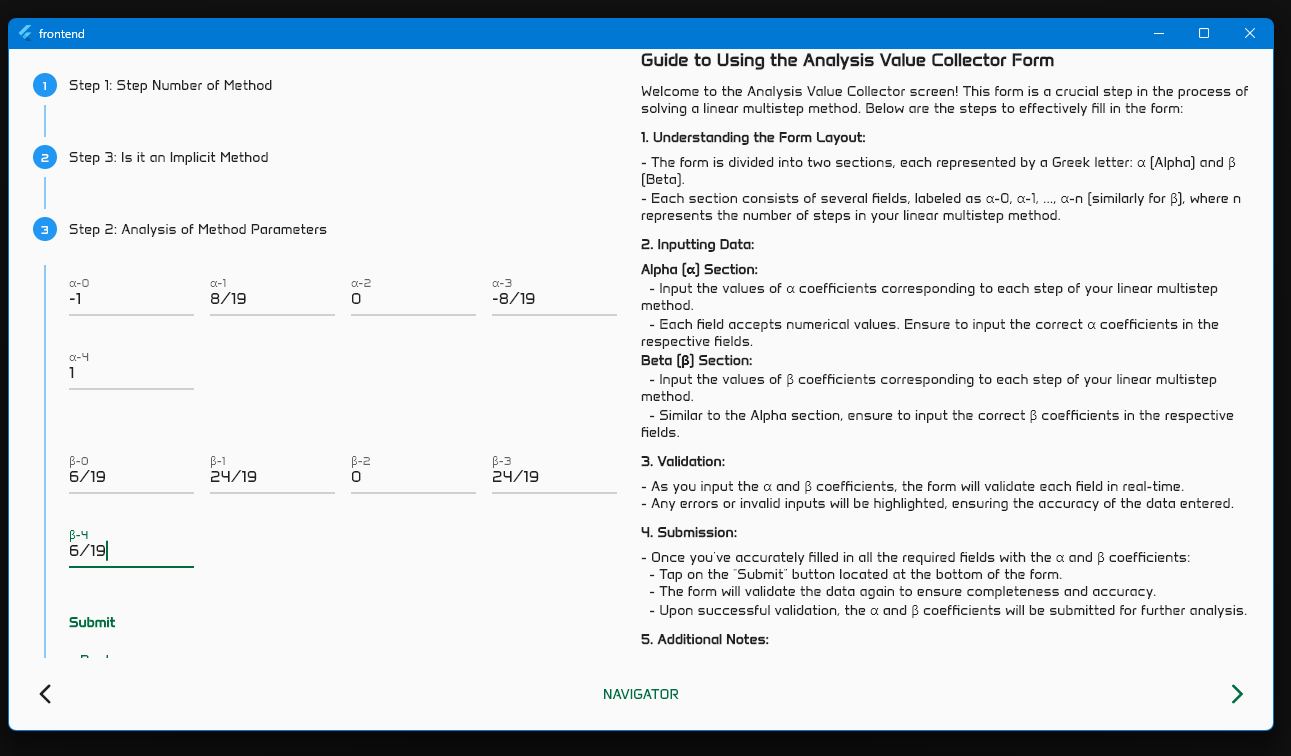
\includegraphics[width=1\textwidth]{chapters/4/image/1.png}
    \caption{$\alpha$ $\beta$ - value collector}
\end{figure}

\begin{figure}[htbp]
    \centering
    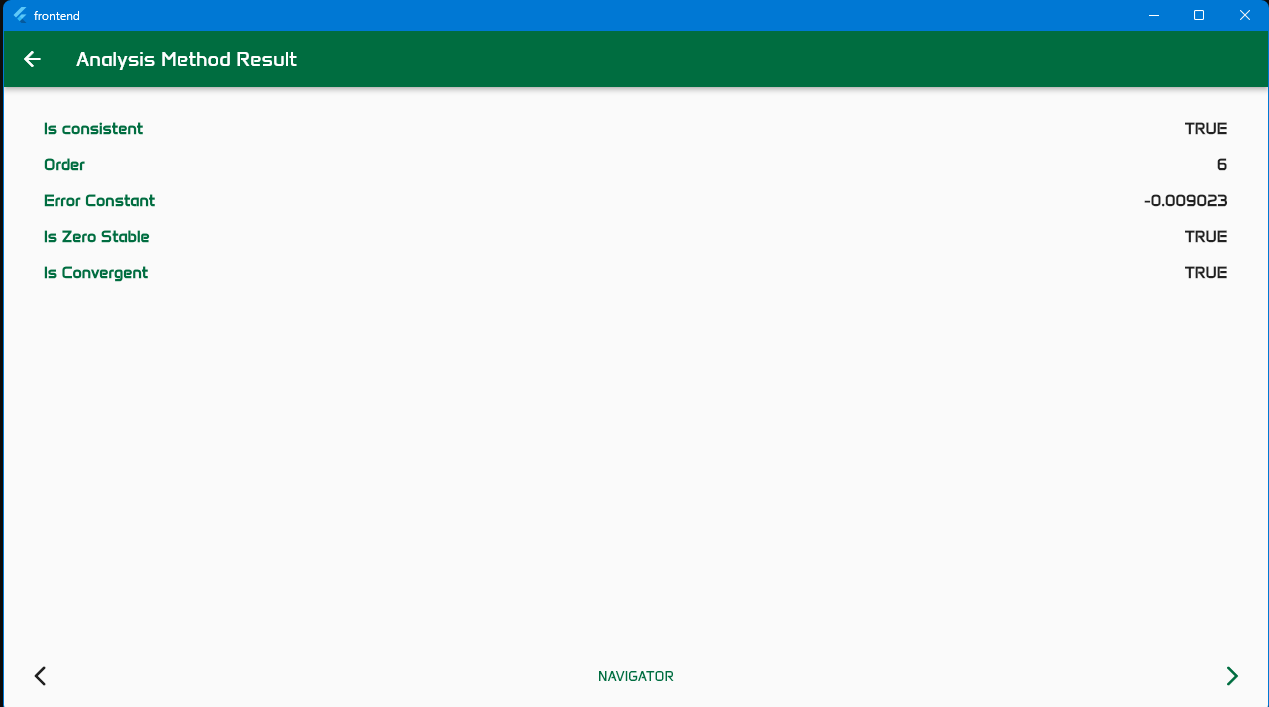
\includegraphics[width=1\textwidth]{chapters/4/image/2.png}
    \caption{Result of Quade's method analysis}
\end{figure}

\newpage

\subsection{3-Step Backward Differentiation Formula}

The 3-Step Backward Differentiation Formula is given as:

\[y_{n+3} = \frac{18}{11} y_{n+2} - \frac{9}{11} y_{n+1} + \frac{2}{11} y_n + \frac{6}{11} h f_{n+3}\]


from the above equation, we can see that the method is a 3-step method,


where:
\[
\begin{aligned}&\alpha_0 &= -\frac{2}{11}, \alpha_1 = \frac{9}{11}, \alpha_2 = -\frac{18}{11}, \alpha_3 = 1 \\
&\beta_0 &= 0, \beta_1 = 0, \beta_2 = 0, \beta_3 = \frac{6}{11}
\end{aligned}
\]

in other to determine the order of the 3-Step BDF's method, we use (3.4), we obtain the following values:

\begin{align}
    c_0 &= \sum_{i=0}^{3} \alpha_i = -\frac{2}{11} + \frac{9}{11} - \frac{18}{11} + 1 = 0 \\
    c_1 &= \sum_{i=0}^{3} (i\alpha_i - \beta_i) = 0 \cdot \alpha_0 + 1 \cdot \alpha_1 + 2 \cdot \alpha_2 + 3 \cdot \alpha_3 - (\beta_0 + \beta_1 + \beta_2 + \beta_3) \nonumber \\
    &= 0 + 1 \cdot \frac{9}{11} + 2 \cdot \left(-\frac{18}{11}\right) + 3 \cdot 1 - \left(0 + 0 + 0 + \frac{6}{11}\right) \nonumber \\
    &= \frac{9}{11} - \frac{36}{11} + 3 - \frac{6}{11} = 0 \\
    c_2 &= \sum_{i=0}^{3} \left(\frac{i^2}{2!} \alpha_i - i \beta_i \right) = \left(\frac{0^2}{2!} \alpha_0 - 0 \cdot \beta_0\right) + \left(\frac{1^2}{2!} \alpha_1 - 1 \cdot \beta_1\right) + \left(\frac{2^2}{2!} \alpha_2 - 2 \cdot \beta_2\right) + \left(\frac{3^2}{2!} \alpha_3 - 3 \cdot \beta_3\right) \nonumber \\
    &= 0 + \frac{1}{2} \cdot \frac{9}{11} - 0 + \frac{4}{2} \cdot \left(-\frac{18}{11}\right) - 0 + \frac{9}{2} \cdot 1 - \frac{18}{11} \nonumber \\
    &= \frac{9}{22} - \frac{36}{11} + \frac{9}{2} - \frac{18}{11} = 0 \\
    c_3 &= \sum_{i=0}^{3} \left(\frac{i^3}{3!} \alpha_i - \frac{i^2}{2!} \beta_i \right) = \left(\frac{0^3}{3!} \alpha_0 - \frac{0^2}{2!} \beta_0\right) + \left(\frac{1^3}{3!} \alpha_1 - \frac{1^2}{2!} \beta_1\right) + \left(\frac{2^3}{3!} \alpha_2 - \frac{2^2}{2!} \beta_2\right) + \left(\frac{3^3}{3!} \alpha_3 - \frac{3^2}{2!} \beta_3\right) \nonumber \\
    &= 0 + \frac{1}{6} \cdot \frac{9}{11} - \frac{1}{2} \cdot 0 + \frac{8}{6} \cdot \left(-\frac{18}{11}\right) - \frac{4}{2} \cdot 0 + \frac{27}{6} \cdot 1 - \frac{9}{2} \cdot \frac{6}{11} \nonumber \\
    &= \frac{9}{66} - \frac{144}{66} + \frac{27}{6} - \frac{54}{11} = 0 \\
    c_4 &= \sum_{i=0}^{3} \left(\frac{i^4}{4!} \alpha_i - \frac{i^3}{3!} \beta_i \right) = \left(\frac{0^4}{4!} \alpha_0 - \frac{0^3}{3!} \beta_0 \right) + \left(\frac{1^4}{4!} \alpha_1 - \frac{1^3}{3!} \beta_1 \right) + \left(\frac{2^4}{4!} \alpha_2 - \frac{2^3}{3!} \beta_2 \right) + \left(\frac{3^4}{4!} \alpha_3 - \frac{3^3}{3!} \beta_3 \right) \nonumber \\
    &= 0 + \frac{1}{24} \cdot \frac{9}{11} - \frac{1}{6} \cdot 0 + \frac{16}{24} \cdot \left(-\frac{18}{11}\right) - \frac{8}{6} \cdot 0 + \frac{81}{24} \cdot 1 - \frac{27}{6} \cdot \frac{6}{11} \nonumber \\
    &= \frac{9}{264} - \frac{288}{264} + \frac{81}{24} - \frac{162}{22} = -\frac{3}{22} = - 0.13636364
\end{align}




The characteristic polynomial \(P(z)\) associated with the BDF-3 method is given by:

\begin{equation}
    P(z) = 11z^3 - 18z^2 + 9z - 2  
\end{equation}



Solving the Algebraic Equation 

\begin{eqnarray}
    11z^3 - 18z^2 + 9z - 2 = 0 \\
    11z^3 - 18z^2 + 9z - 2 = (z - 1)(11z^2 - 7z + 2) \\    
    11z^2 - 7z + 2 = 0 \\
    (z - 1) = 0 \\
    z = \frac{7 \pm \sqrt{(-7)^2 - 4(11)(2)}}{2(11)} = \frac{7 \pm \sqrt{49 - 88}}{22} = \frac{7 \pm i\sqrt{39}}{22} 
\end{eqnarray}

Therefore, the roots of the polynomial \(11z^3 - 18z^2 + 9z - 2 = 0\) are:

\begin{eqnarray}
    z = 1 \\
    z = \frac{7 + i\sqrt{39}}{22} \\
    z = \frac{7 - i\sqrt{39}}{22}
\end{eqnarray}
We take the modulus of the roots to check for zero-stability:
\begin{eqnarray}
    |z| = |1| = 1 \\
    |z| = \sqrt{\left(\frac{7}{22}\right)^2 + \left(\frac{\sqrt{39}}{22}\right)^2} = \sqrt{\frac{49}{484} + \frac{39}{484}} = \sqrt{\frac{88}{484}} = \sqrt{\frac{22}{121}} = \frac{\sqrt{22}}{11} < 1 \\
    |z| = \sqrt{\left(\frac{7}{22}\right)^2 + \left(-\frac{\sqrt{39}}{22}\right)^2} = \sqrt{\frac{49}{484} + \frac{39}{484}} = \sqrt{\frac{88}{484}} = \sqrt{\frac{22}{121}} = \frac{\sqrt{22}}{11} < 1
\end{eqnarray}

Using Equation (3.4), we can see that the method is a 3-step method of order 3. The method is consistent since \(c_0 = 0\) and \(c_1 = 0\). Furthermore, the method is zero-stable since the roots of the characteristic equation are all inside the unit circle. Lastly, the method is convergent since the error constant is \(-\frac{3}{22}\) or approximately \(-0.1363634\).

Using the JF-Solver to analyze the 3-step Backward Differentiation Formula (BDF(3)), we obtain the following results as shown below:

\begin{figure}[htbp]
    \centering
    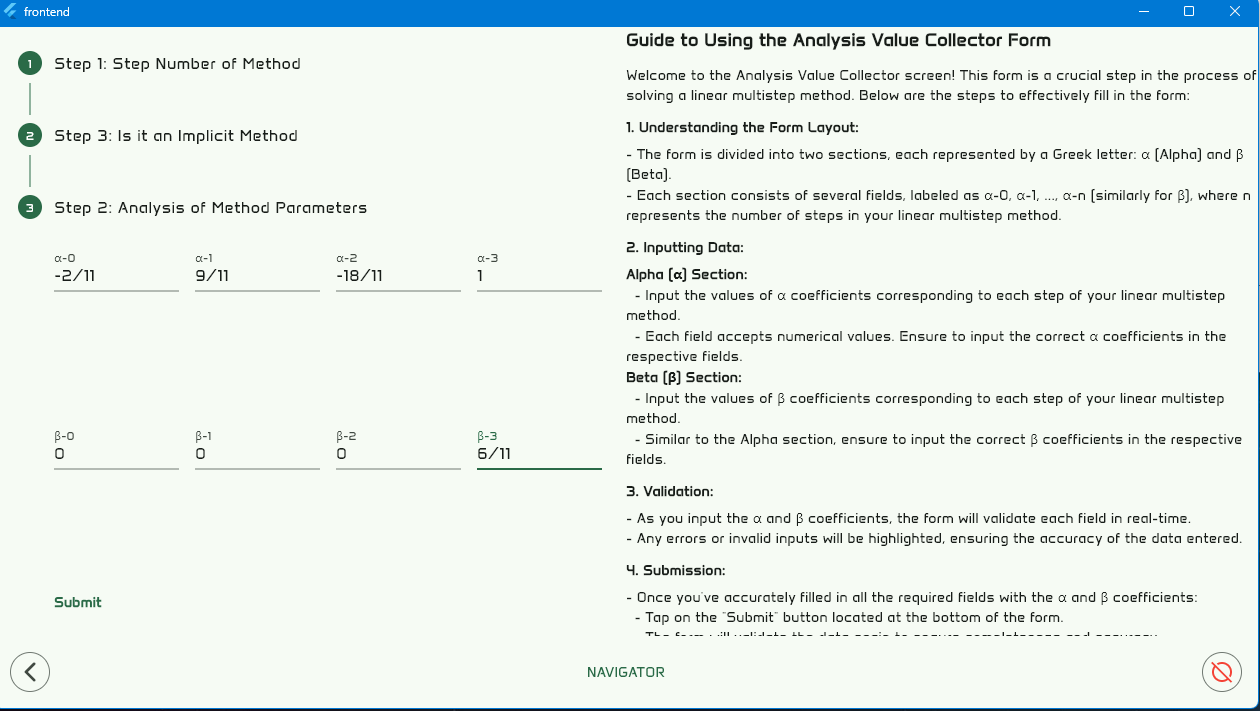
\includegraphics[width=1\textwidth]{chapters/4/image/5.png}
    \caption{$\alpha$ $\beta$ - value collector for 3-step BDF method}
\end{figure}

\begin{figure}[htbp]
    \centering
    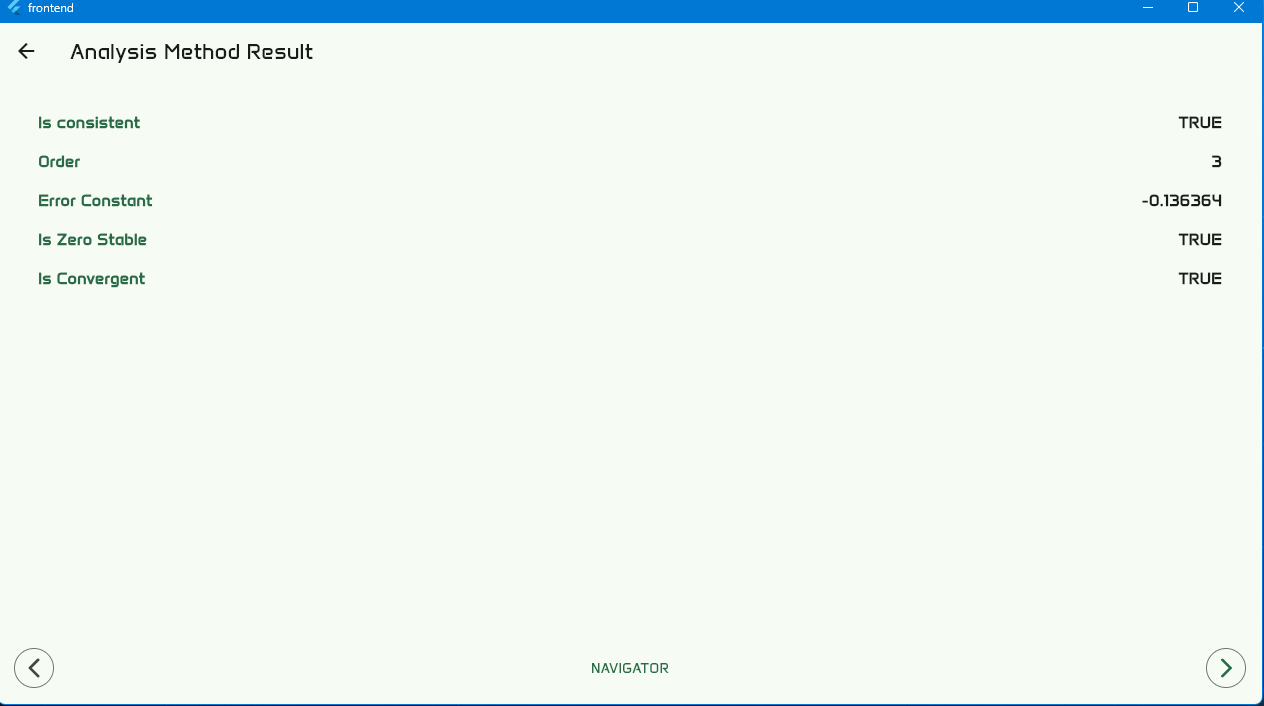
\includegraphics[width=1\textwidth]{chapters/4/image/6.png}
    \caption{Results of the 3-step BDF method analysis}
\end{figure}

Additionally, the JF-Solver software, which was developed as part of this research, has been used to analyze the BDF(3) method. The software successfully replicated the theoretical results, providing the same error constant and stability characteristics. Moreover, the JF-Solver demonstrated superior performance in terms of computation speed and efficiency, making it a valuable tool for numerical analysis of differential equations.


%! Module 2: Solving Differential Equations

% \newpage
\section{Module 2: Solving Differential Equations}

\subsection{Explicit Method: Adams-Bashforth Method 3-Step Method}
Consider the problem \begin{equation}
    f(x,y) = 3x^2y
\end{equation}, with the initial condition $y(0) = 1$, the step-size also given as $h = 0.1$.

The Adams-Bashforth 3-step method is given as:
\begin{equation}
    y_{n+3}  = y_{n+2} + h \left(\frac{23}{12}f_{n+2} - \frac{4}{3}f_{n+1} + \frac{5}{12}f_{n}\right)
\end{equation}

The exact solution to the problem is given as:
\begin{equation}
    y(x) = e^{x^3}
\end{equation}




\begin{table}[htbp]
    \centering
    \begin{tabular}{|c|c|c|c|}
        \hline
        Step $n$ & Adams-Bashforth 3-step Method & JF-Solver & Exact Value \\
        \hline
        $y_0$ & 1.000000 & 1.000000 & 1.000000 \\
        $y_1$ & 1.001000 & 1.001000 & 1.001001 \\
        $y_2$ & 1.008032 & 1.008032 & 1.008032 \\
        $y_3$ & 1.027213 & 1.027213 & 1.027398 \\
        $y_4$ & 1.065494 & 1.065494 & 1.066492 \\
        $y_5$ & 1.131580 & 1.131580 & 1.133148 \\
        $y_6$ & 1.237609 & 1.237609 & 1.241857 \\
        $y_7$ & 1.401946 & 1.401946 & 1.409637 \\
        $y_8$ & 1.654090 & 1.654090 & 1.669859 \\
        $y_9$ & 2.043706 & 2.043706 & 2.073784 \\
        \hline
    \end{tabular}
    \caption{Comparison of Results: Adams-Bashforth 3-step Method, JF-Solver, and Exact Values}
    \label{tab:comparison}
\end{table}


The table illustrates the numerical values obtained at each step $n$. The Adams-Bashforth 3-step method and the JF-Solver results are compared against the exact solution $y = e^{x^3}$.

The images below shows that output of the JF-Solver:

\begin{figure}[htbp]
    \centering
    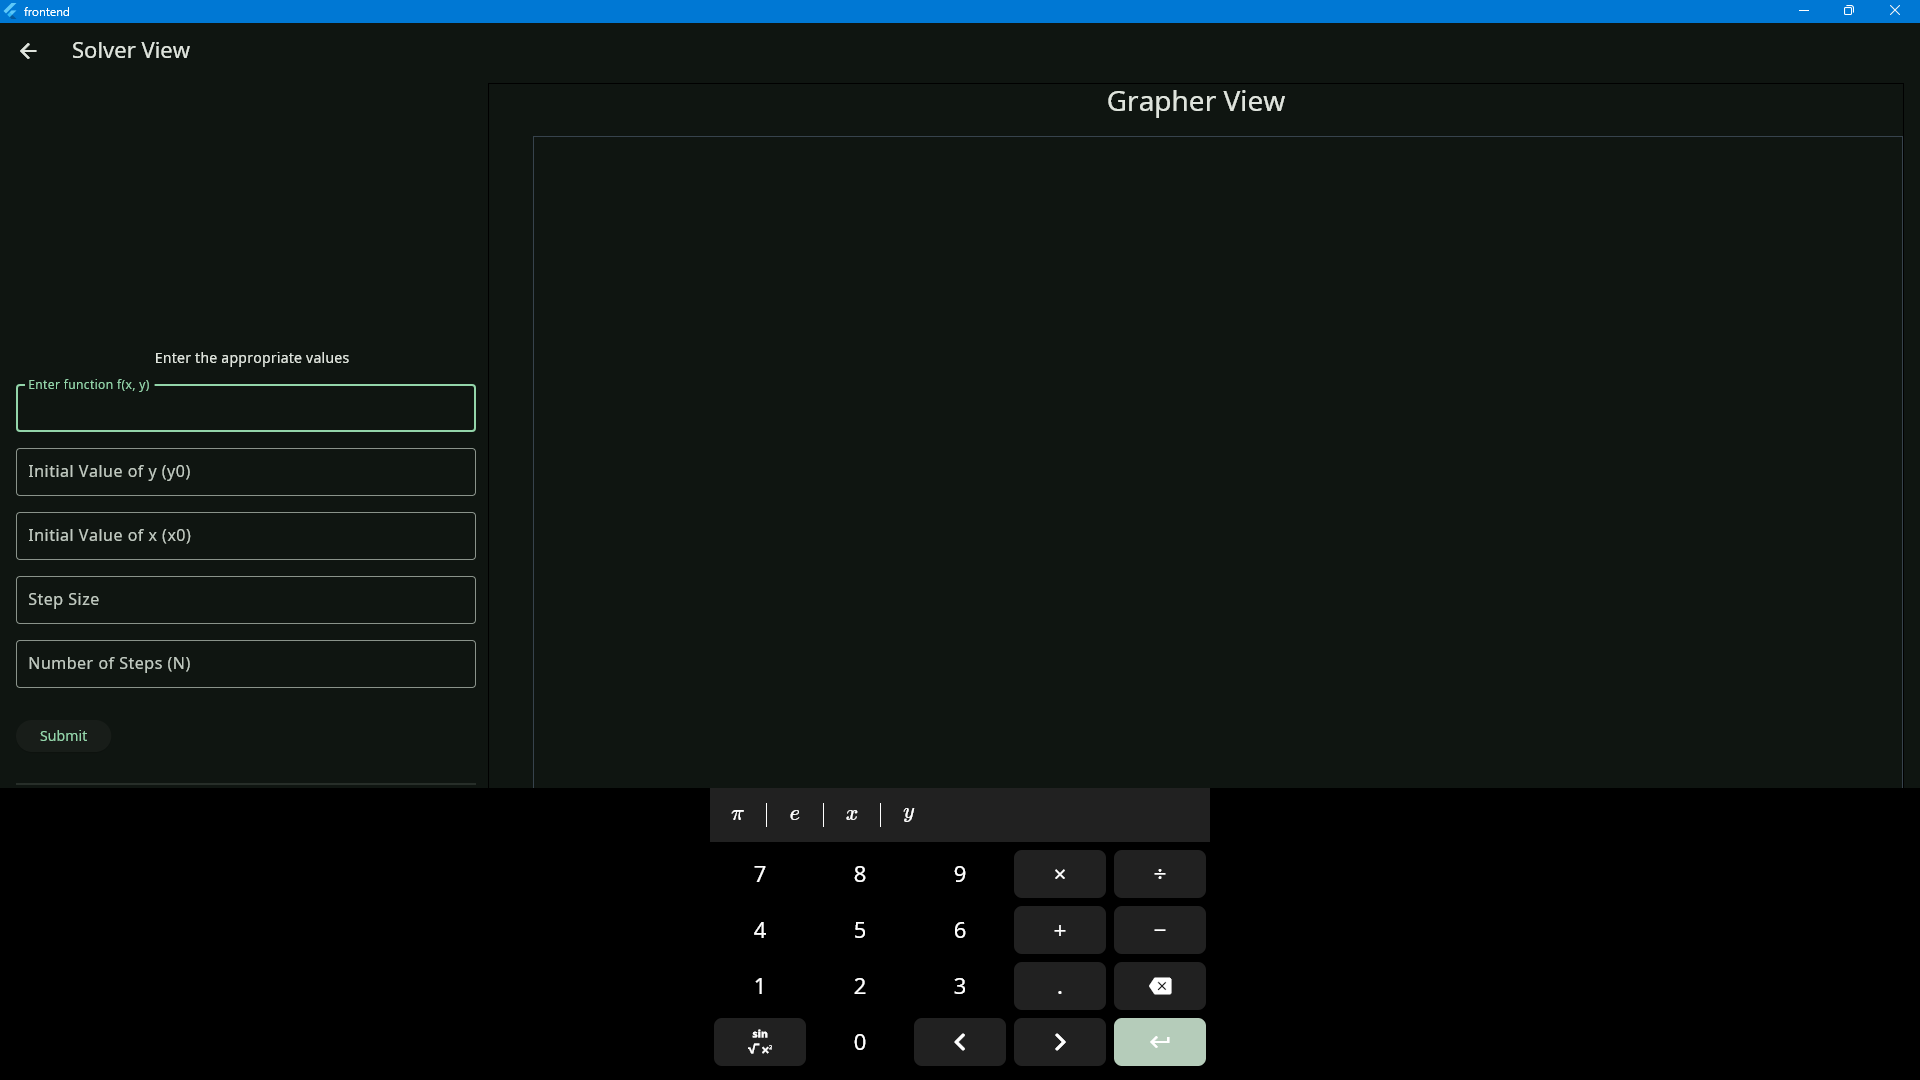
\includegraphics[width=1\textwidth]{chapters/4/image/solver_3.png}
    \caption{The JF-Solver view}
\end{figure}

\begin{figure}[htbp]
    \centering
    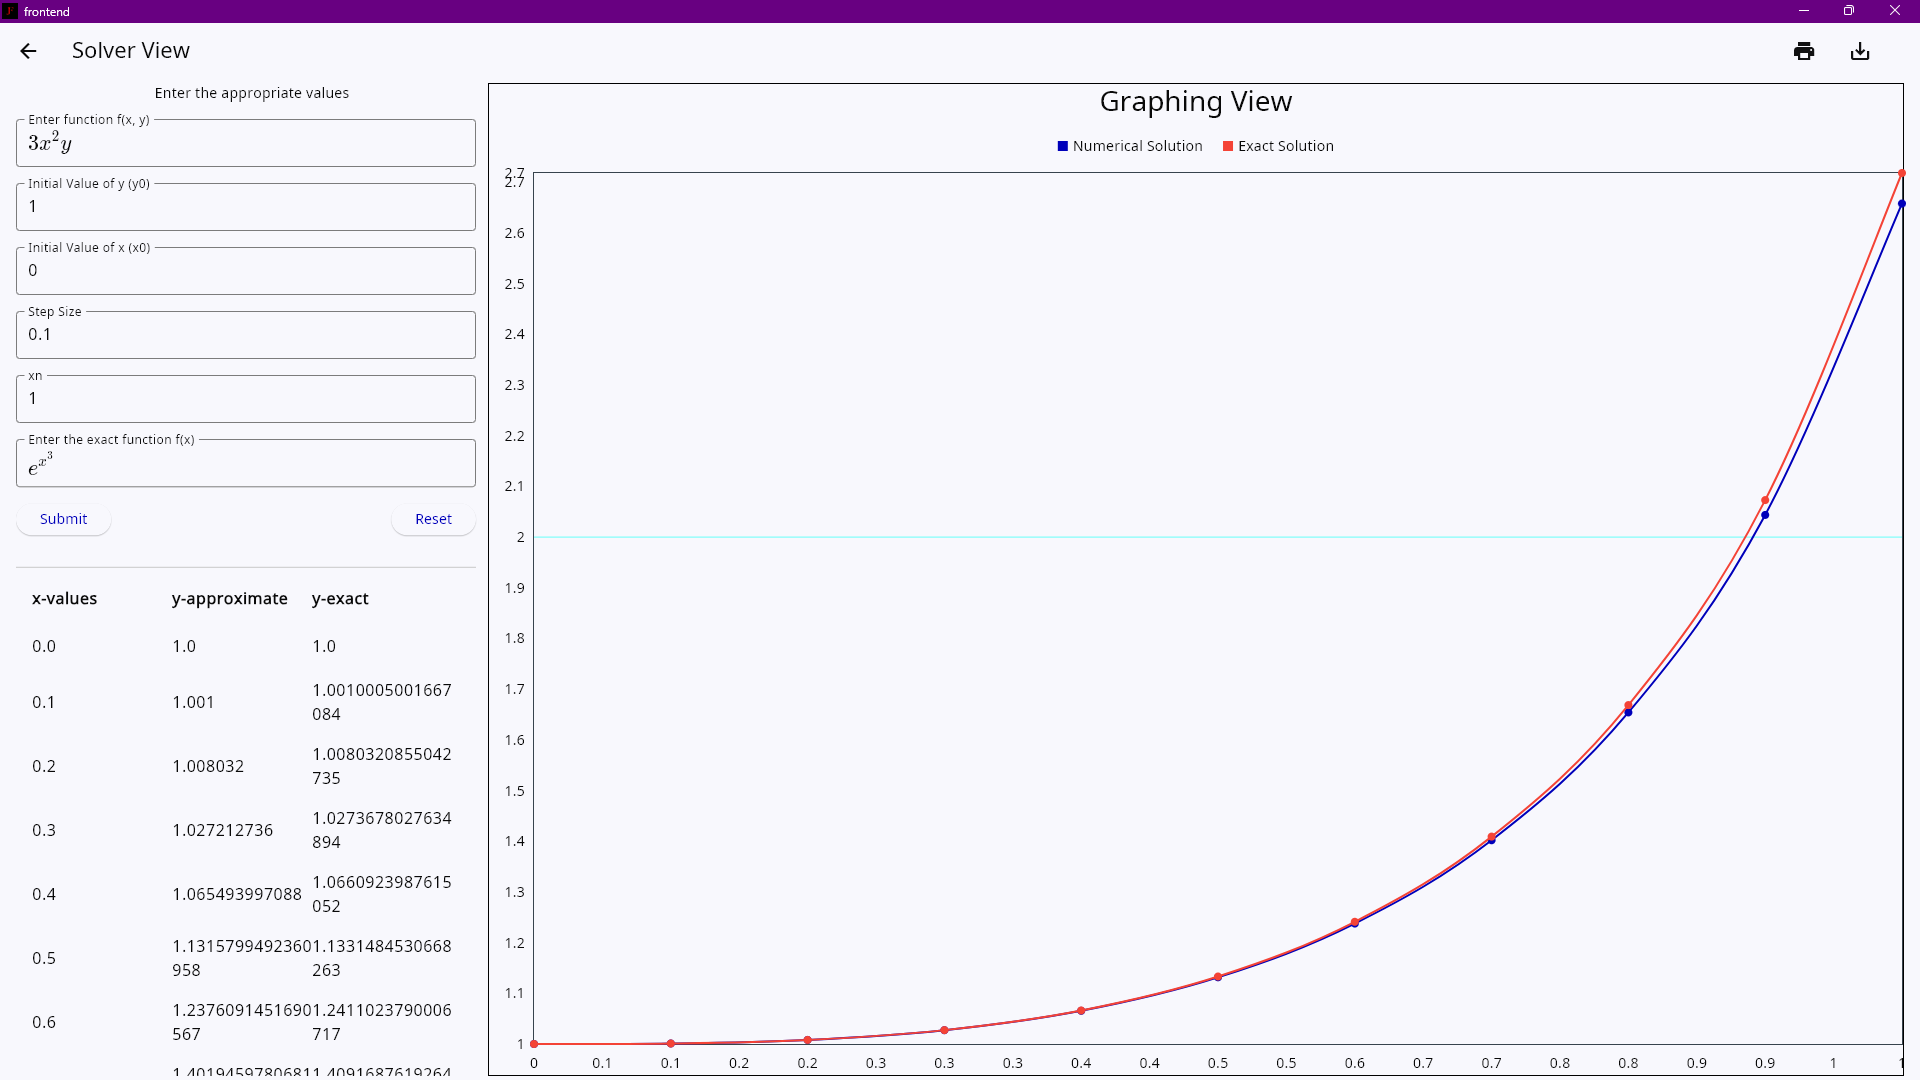
\includegraphics[width=1\textwidth]{chapters/4/image/solver_2.png}
    \caption{output result of the JF-Solver for $(4.30)$ }
\end{figure}


\newpage
From the comparison, it is evident that both the Adams-Bashforth 3-step method and the JF-Solver produce results that closely approximate the exact solution. The JF-Solver results are rounded to six decimal places, showing a high degree of accuracy.

This comparison demonstrates the effectiveness, accuracy, and reliability of the JF-Solver in approximating the solution of explicit differential equations using the Linear Multistep Method (LMM) given. The application works by accepting the coefficients of the LMM and then solves the differential equation using these coefficients.

\section{Implicit Method(Predictor-Corrector Algorithm): Adams-Moulton Method 4-Step Method (Stiff problem)}


\section{Implicit Method(Linearization Algorithm): Adams-Moulton Method 4-Step Method (Stiff problem)}




\chapter{Summary and Conclusion}
\section{Summary}

\bibliographystyle{apacite}
\bibliography{bib/Proposal} 
% Include your bibliography file (e.g., references.bib)

\end{document}
